%%%%%%%%%%%%%%%%%%%%%%%%%%%%%%%%%%%%%%%%%
% Simple Sectioned Essay Template
% LaTeX Template
%
% This template has been downloaded from:
% http://www.latextemplates.com
%
% Note:
% The \lipsum[#] commands throughout this template generate dummy text
% to fill the template out. These commands should all be removed when 
% writing essay content.
%
%%%%%%%%%%%%%%%%%%%%%%%%%%%%%%%%%%%%%%%%%

%----------------------------------------------------------------------------------------
%	PACKAGES AND OTHER DOCUMENT CONFIGURATIONS
%----------------------------------------------------------------------------------------

\documentclass[5pt]{article} % Default font size is 12pt, it can be changed here

\usepackage{geometry} % Required to change the page size to A4
\geometry{a4paper} % Set the page size to be A4 as opposed to the default US Letter

\usepackage{graphicx} % Required for including pictures

\usepackage{float} % Allows putting an [H] in \begin{figure} to specify the exact location of the figure
\usepackage{wrapfig} % Allows in-line images such as the example fish picture
\usepackage{hyperref}
\usepackage{caption}
\usepackage{subcaption}
\usepackage{rotating}

\usepackage{lipsum} % Used for inserting dummy 'Lorem ipsum' text into the template

\linespread{1.2} % Line spacing

%\setlength\parindent{0pt} % Uncomment to remove all indentation from paragraphs

\graphicspath{{images/}} % Specifies the directory where pictures are stored

\begin{document}

%----------------------------------------------------------------------------------------
%	TITLE PAGE
%----------------------------------------------------------------------------------------

\begin{titlepage}

\newcommand{\HRule}{\rule{\linewidth}{0.5mm}} % Defines a new command for the horizontal lines, change thickness here

\center % Center everything on the page

%\textsc{\LARGE CS 420: Team Project 2}\\[1.5cm] % Name of your university/college
\textsc{\Large Human Computer Interface and Design}\\[0.5cm] % Major heading such as course name
\textsc{\large College of William \& Mary}\\[0.5cm] % Minor heading such as course title

\HRule \\[0.4cm]
{ \huge \bfseries CS 420: Team Project 2}\\[0.4cm] % Title of your document
\HRule \\[1.5cm]

\begin{minipage}{0.4\textwidth}
\begin{flushleft} \large
\emph{Authors:}\\
Derek O'Connell \\
Alexander Powell \\
John Sawin \\
Thomas Van de Houten
\end{flushleft}
\end{minipage}
~
\begin{minipage}{0.4\textwidth}
\begin{flushright} \large
\end{flushright}
\end{minipage}\\[4cm]

{\large \today}\\[3cm] % Date, change the \today to a set date if you want to be precise

%\includegraphics{Logo}\\[1cm] % Include a department/university logo - this will require the graphicx package

\vfill % Fill the rest of the page with whitespace

\end{titlepage}

\section{Personas}

\begin{itemize}
\item Sources
\begin{itemize}
\item John J. Byxbe - Associate Director of Auxiliary Services (private meeting on 3/28)
\item \url{https://colleges.niche.com/college-of-william--and--mary/statistics/}
\item \url{http://www.collegetuitioncompare.com/edu/231624/college-of-william-and-mary/enrollment/}
\end{itemize}
\item Data
\begin{itemize}
\item Meal Plans for spring 2016 total 5376 students (from Byxbe meeting)
\begin{itemize}
\item 1492 on Gold 19
\item 196 on Freedom
\item 1954 on Gold 14
\item 603 on Block 125
\item 561 on Block 100
\item 1 on Block 20
\item 569 on Commuter
\end{itemize}
\item Students are mostly ages 18-24. There are about 700 students between 25 and 30 and 44 students are younger than 18.
\item The students are 55\% female and 45\% male
\item 62\% of students are white, 7.5\% are unspecified, 8\% are Asian, 7\% are black
\item 25\% of students are in a social fraternity
\item 85\% of undergraduates participate in varsity, club, or intramural sports.
\item 40\% of students receive no financial aid, 22\% are using Institutional grants, 20\% are on students loans.
\item 65\% Of students are from Virginia
\item Business is the most popular major department.
\item 2.5\% of students are transfers
\item 96\% of students are regular, full-time students.
\item 81\% of students were in the top 10\% of their high school class.
\end{itemize}
\end{itemize}

\center{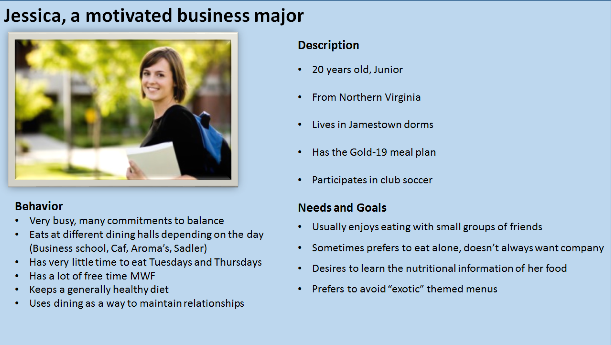
\includegraphics[width=1\linewidth]{jessica_persona}}

\subsection{Assumptions}
\begin{itemize}
\item Traits like usually eating with groups of small friends and occasionally eating alone are traits that I commonly witness and experience for myself while at W\&M. 
\item Desiring to know nutritional information is assumed since most students participate in some sort of physical activity, and have some consciousness about their nutrition. 
\item The ``exotic" themed food represents an idiosyncrasy of a random student. Others might include food allergies, vegetarianism, veganism, or religious diets. Because of the abundance of very specific diets, it is reasonable to apply some sort of trait to this persona. 
\end{itemize}
\subsection{Rationale for each characteristic}
\begin{itemize}
\item Between 18 and 22: This is the most common age group for undergraduate students.  
\item From Northern Virginia: This is the most common home location for undergraduate students.  
\item Excelled in High School, in the top of her class: Data straight from the websites, reflects her initiative and goal setting
\item From an upper-middle class family: Reflects and impact on her world-view, which can impact patience when dealing
\item Participates in club soccer: Demonstrates that she has other personal investments outside of school
\end{itemize}

\center{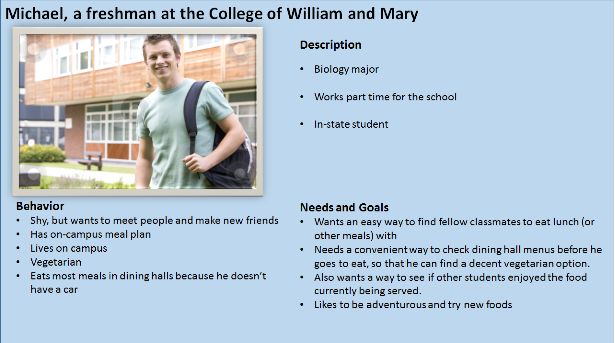
\includegraphics[width=1\linewidth]{michael_persona}}

\subsection{Assumptions and their rationale}
\begin{itemize}
\item The shyness is based off of a typical WM student. Walking around campus, one easily notices that most students are quiet and keep to themselves, but are warm and friendly if prompted.
\item About 70\% of the student body lives on campus. Meal plans are mandatory for on-campus student. It is then justified that he should have a meal plan. 
\item The vegetarian trait reflects the “Meatless Mondays” and anti-meat trends occurring at William and Mary. 
\item Freshman are not allowed to have cars on campus, explaining why he does not have car, and eats most meals at dining halls. 
\item His major, Biology, is a natural science, the second most common major at William and Mary. 
\item He is an in-state student, reflecting the most common type of student. 
\item He works part-time. While this isn’t the norm, a large amount of students do work part-time. He represents a large subset of the student population. 
\item His adventurous taste for new foods represents the globally-minded view of the typical William and Mary student. A large number of students travel abroad and are exposed to new cuisine. An even larger number of students are exposed to other cultures through friends and classes. 
\end{itemize}

\section{Use Case}

\center{\fbox{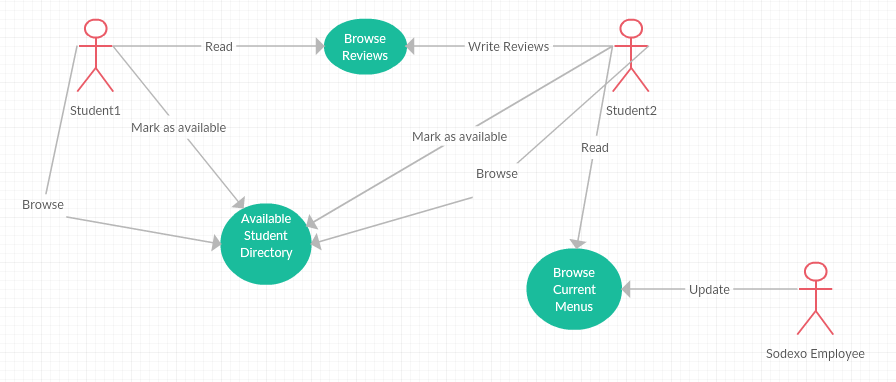
\includegraphics[width=1\linewidth]{UseCase1}}}

\begin{flushleft}
The use case diagram for EatWithFriends contains three main use cases.  These are the ability to browse dining hall menus, browse reviews about the food from other students as well as post your own, and most importantly, find other friends to eat with.  We included several different actors in our use case diagram.  For the sake of simplicity, we used two students to illustrate how one student can perform actions like post a review of the meal they just had, and another student can read it and change their decision of where they want to eat.  Additionally, we include W\&M Dining/Sodexo as an actor because for the menu portion of the application to be successful, they will need to keep their dining hall menus up to date.
\end{flushleft}

\section{Scenarios}

\begin{enumerate}
\item Scenario 1:
\begin{itemize}
\item Michael (the W\&M freshman from the Persona above) has just gotten out of his intro biology class at 12 o’clock noon.  Since it’s the beginning of the semester and he’s a freshman, Michael doesn’t have a lot of friends he feels comfortable texting to join him for lunch.  
\item Instead, he opens up EatWithFriends on his phone and sees that there are 7 other students on campus who are also looking for someone to eat with.  He recognizes one of the names from his chemistry lab and sends them a message through the app, asking if they would like to join him for lunch.  
\item As a vegetarian, he also checks the menus for the Commons and Sadler center, the two main dining halls on campus.  Seeing that the Commons is serving a vegetarian Indian dish and Sadler is serving hamburgers, he suggests they meet at the Commons in 5 minutes.  
\item Michael and his new friend have a great meal on campus.  Afterwards, Michael leaves a positive reviews of his meal.  
\end{itemize}
\item Scenario 2:
\begin{itemize}
\item Jessica just got back from an all-weekend club-soccer tournament at 5:30 pm on a Sunday evening. She is extremely hungry from the long drive. After a long weekend with her team, she would like to have a social dinner, but doesn’t want to spend any more time with her soccer teammates. It’s still early for dinner, so her roommate, her typical companion for meals, is not ready for dinner. 
\item Jessica uses EatWithFriends to check the menus and reviews at Sadler Center and the Caf. It turns out that the Caf is doing a theme night for German food, and Caf-goers have posted that the eintopf is particularly potent. She decides that she wants to avoid the German cuisine and will go to Sadler.
\item Jessica updates EatWithFriends, and all her friends can see that she is headed to eat at Sadler. Her friend, Suzi, who lives across campus, was also in the mood for dinner, and tells Jessica that she will meet her there. 
\item Jessica and Suzi enjoy a breathtaking meal of hamburgers and french fries at Sadler Center. Halfway through their meal, Justin, a close friend of Suzi’s, joins the two women. Justin, famished from his hot yoga class, used EatWithFriends to learn that the girls were currently eating at Sader Center, he rushed over immediately to join them. Jessica, particularly fond of the night’s meat-patties, writes a haiku about them and posts it to the EatWithFriends public boards. 
\end{itemize}
\end{enumerate}

\newpage
\section{Storyboards}
\begin{figure}[h]
\center{\fbox{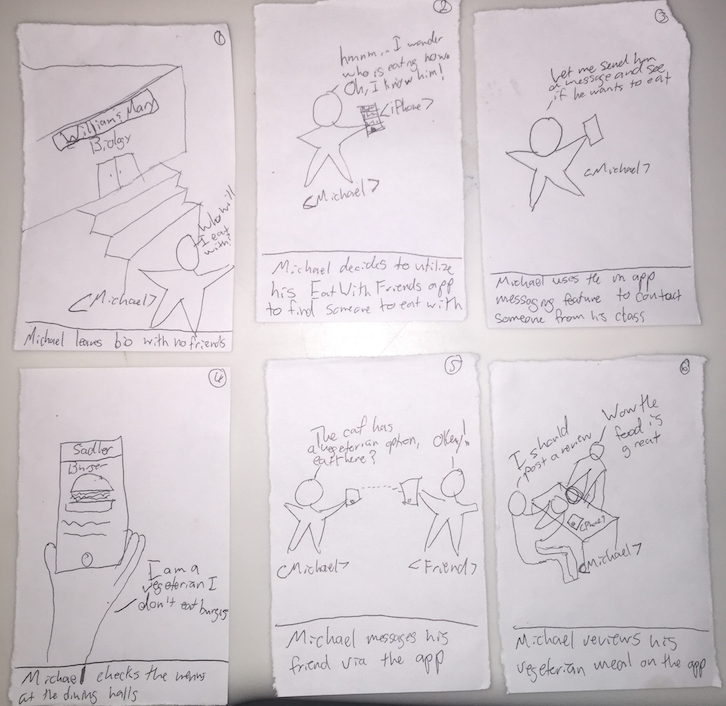
\includegraphics[width=1\linewidth]{Topic4Part1}}}
\caption{Storyboard 1}
\end{figure}
\begin{figure}[h]
\center{\fbox{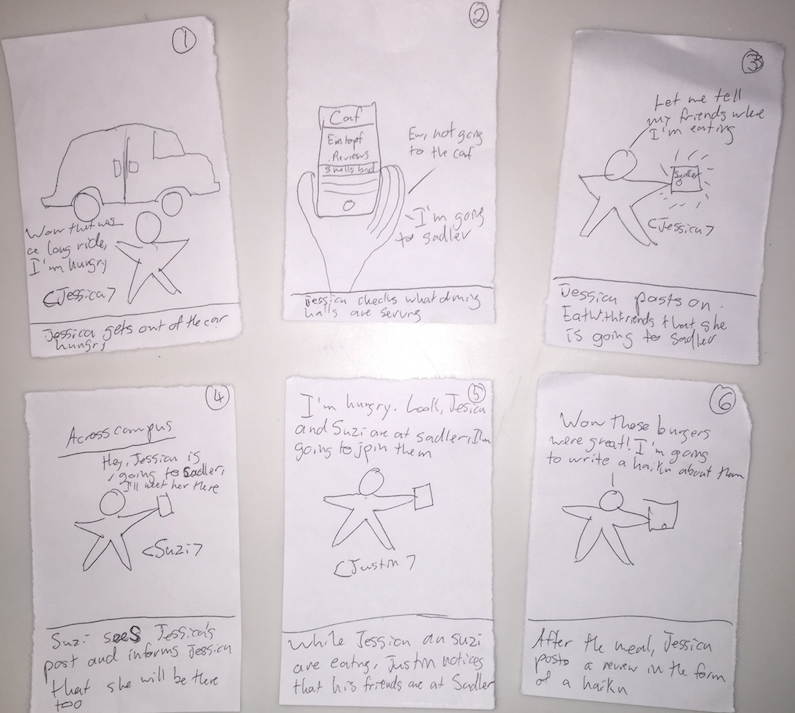
\includegraphics[width=1\linewidth]{Topic4Part2}}}
\caption{Storyboard 1}
\end{figure}
%\clearpage

\newpage
\section{Task Models}
\begin{figure}[h]
\centering
\begin{subfigure}{.5\textwidth}
\fbox{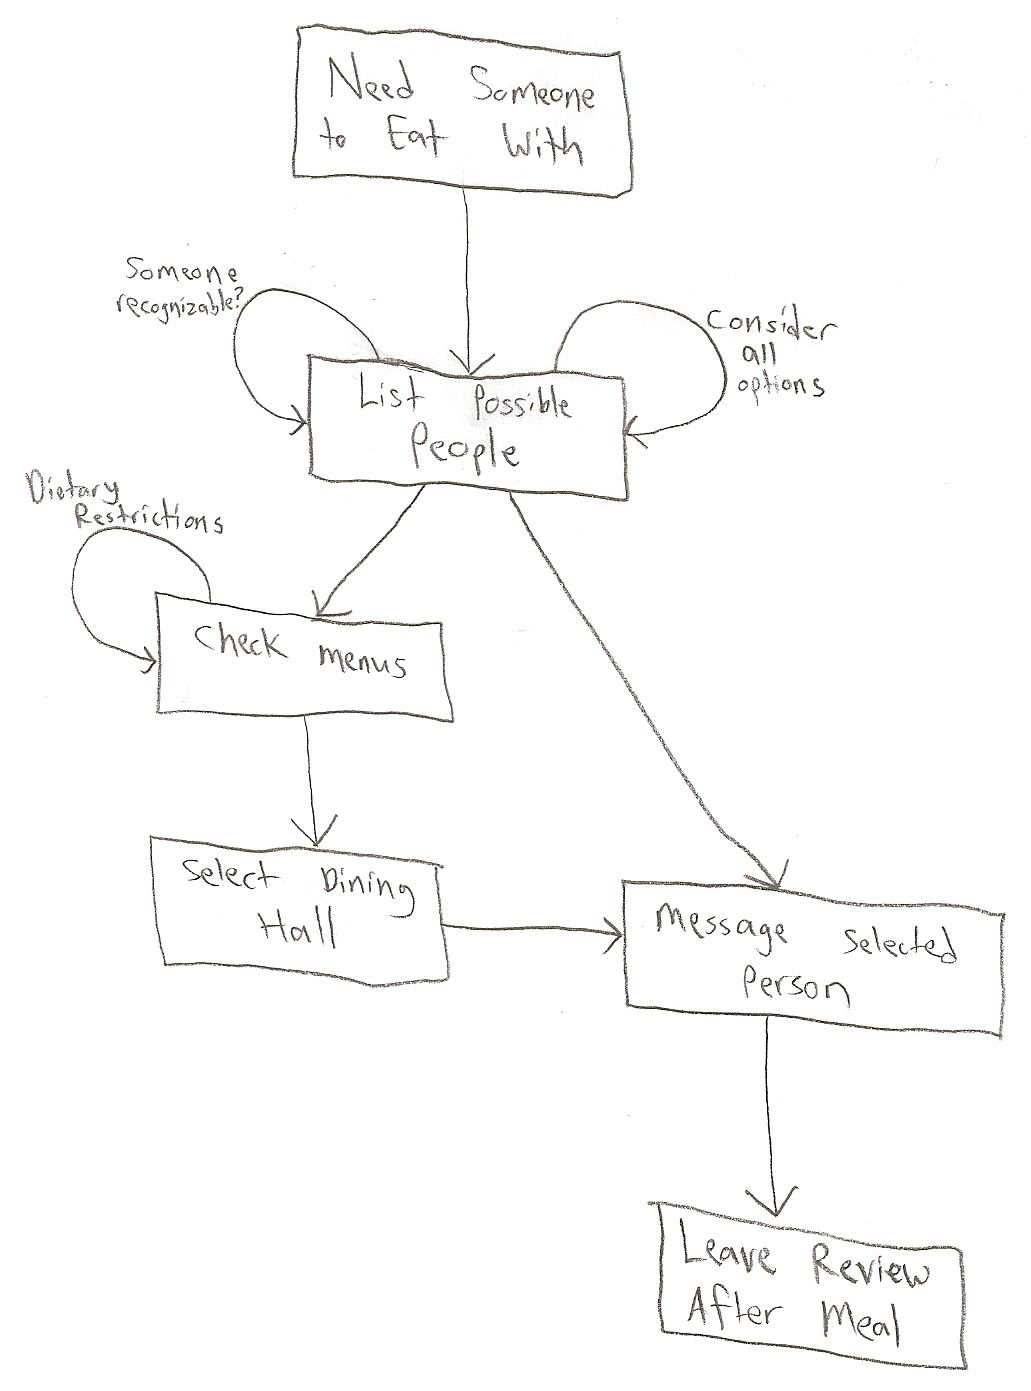
\includegraphics[width=1\linewidth]{Topic5Part1.jpg}}
\caption{Task Model 1}
\end{subfigure}
\begin{subfigure}{.5\textwidth}
\fbox{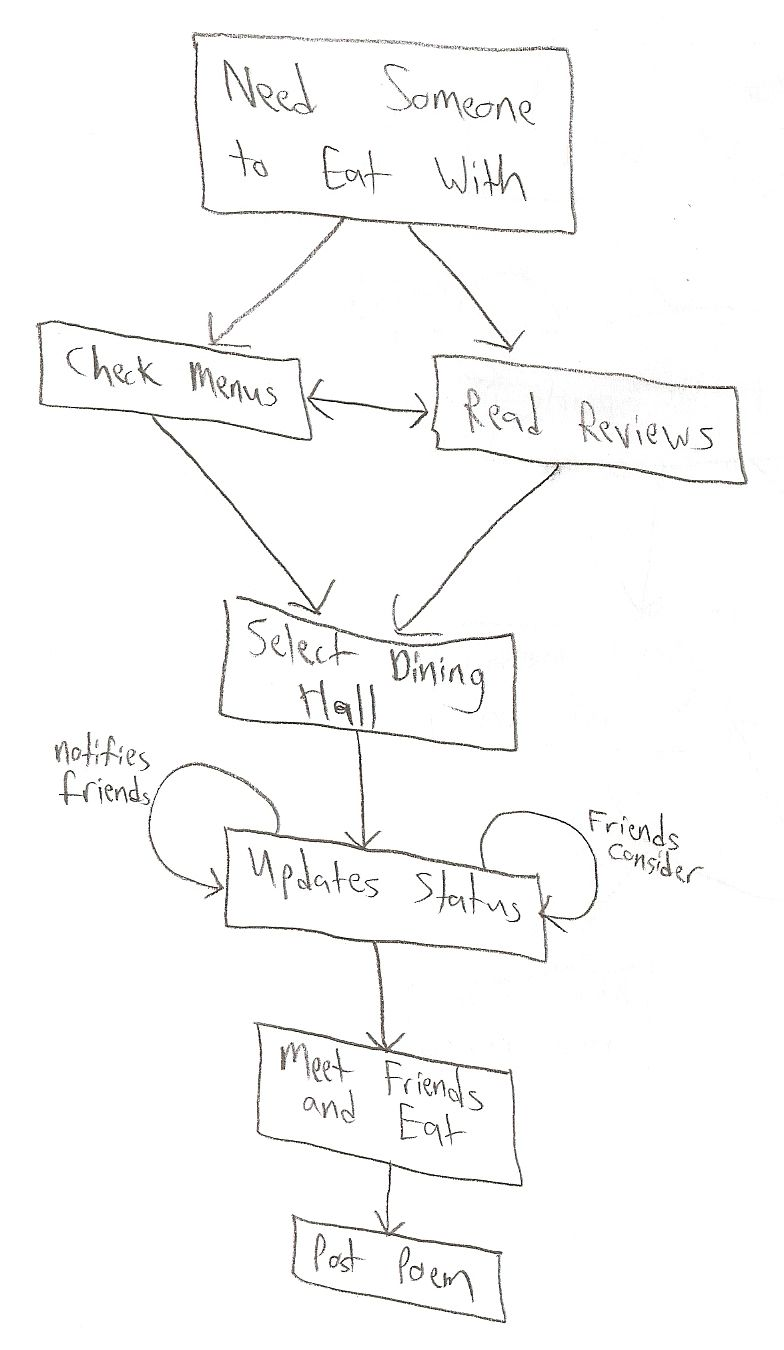
\includegraphics[width=1\linewidth]{Topic5Part2.jpg}}
\caption{Task Model 2}
\end{subfigure}
\end{figure}

\clearpage
\section{Evaluation}

\begin{enumerate}
\item Scenarios
\begin{itemize}
\item Pros
\begin{enumerate}
\item Personal aspect, allows designers to relate to users.  
\item With scenarios, you have the ability to dive deep into a specific aspect of the project, and really show how the user would interact with it.  
\item Require the development of personas, which in turn require research into the user-population, yielding UX-relevant info. 
\end{enumerate}
\item Cons
\begin{enumerate}
\item The limited number of scenarios prevents developers from covering every possible use.  
\item Focus on the best-case can might encourage the development of unstable software, or UX that is unfriendly for those without specific goals.
\end{enumerate}
\end{itemize}
\item Storyboards
\begin{itemize}
\item Pros
\begin{enumerate}
\item Relatable, as it provides visual representation of the scenario.  
\item Quick to draw up, as detailing a UI is unnecessary for a fully functioning storyboard.  
\item Can highlight specific aspects of the scenario and persona as necessary.  
\end{enumerate}
\item Cons
\begin{enumerate}
\item Artistic ability can limit functionality
\end{enumerate}
\end{itemize}
\item Task Models
\begin{itemize}
\item Pros
\begin{enumerate}
\item Relatively quick to create, no frills.  
\item Can strategically and efficiently display all possible user interactions with the project.
\end{enumerate}
\item Cons
\begin{enumerate}
\item Not much personality or relatability.  
\end{enumerate}
\end{itemize}
\end{enumerate}

\subsection{Summary}
The scenario serves as the backbone for the storyboards and task models. Detailed scenarios also allow for storyboards and task models to be quickly developed. However it further depth of the storyboards and task models that gives the UX team the necessary insight for a ``killer UX". Storyboards are linear, so they provide a chronological representation of potential application usage in real-world scenarios. Task models on the other hand are more abstract, they show all possible actions from a certain state within the UX, regardless of some specific scenario. 

\newpage
\section{Ideas per Participant}

\begin{figure}[h!]
\centering
\fbox{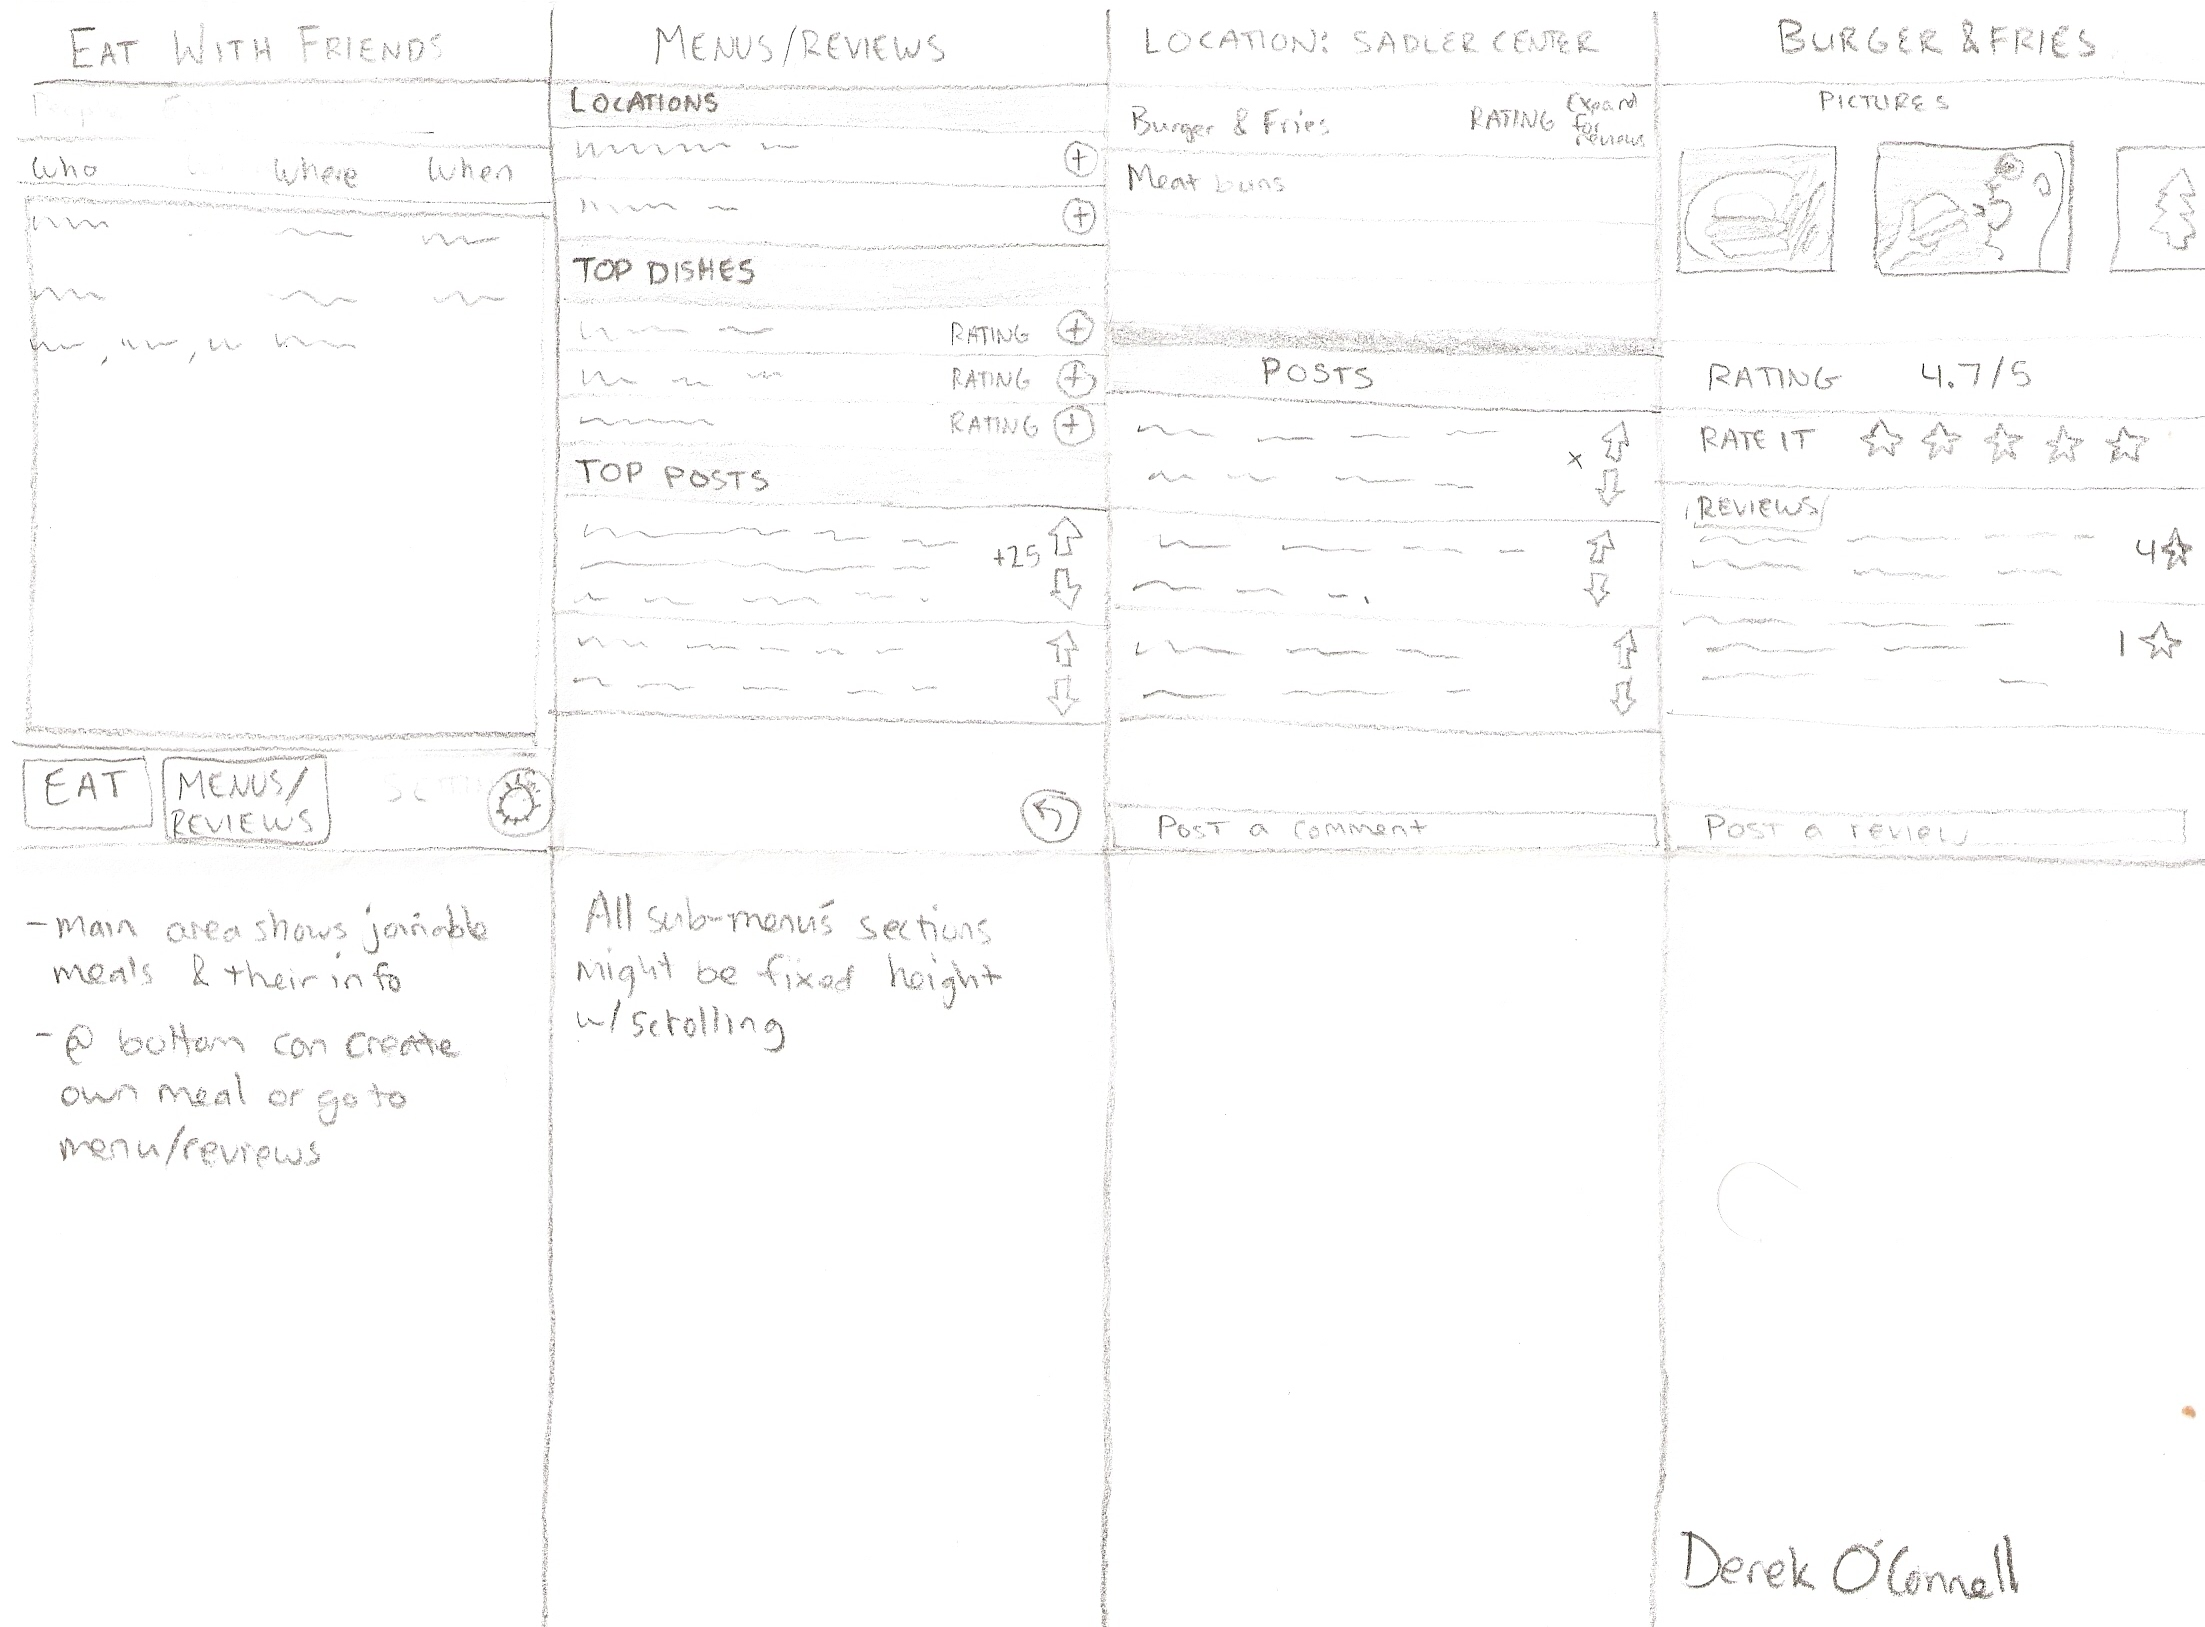
\includegraphics[width=0.8\linewidth]{derek1.jpg}}
\caption{6 Ideas from Derek}
\end{figure}

\begin{figure}[h!]
\centering
\fbox{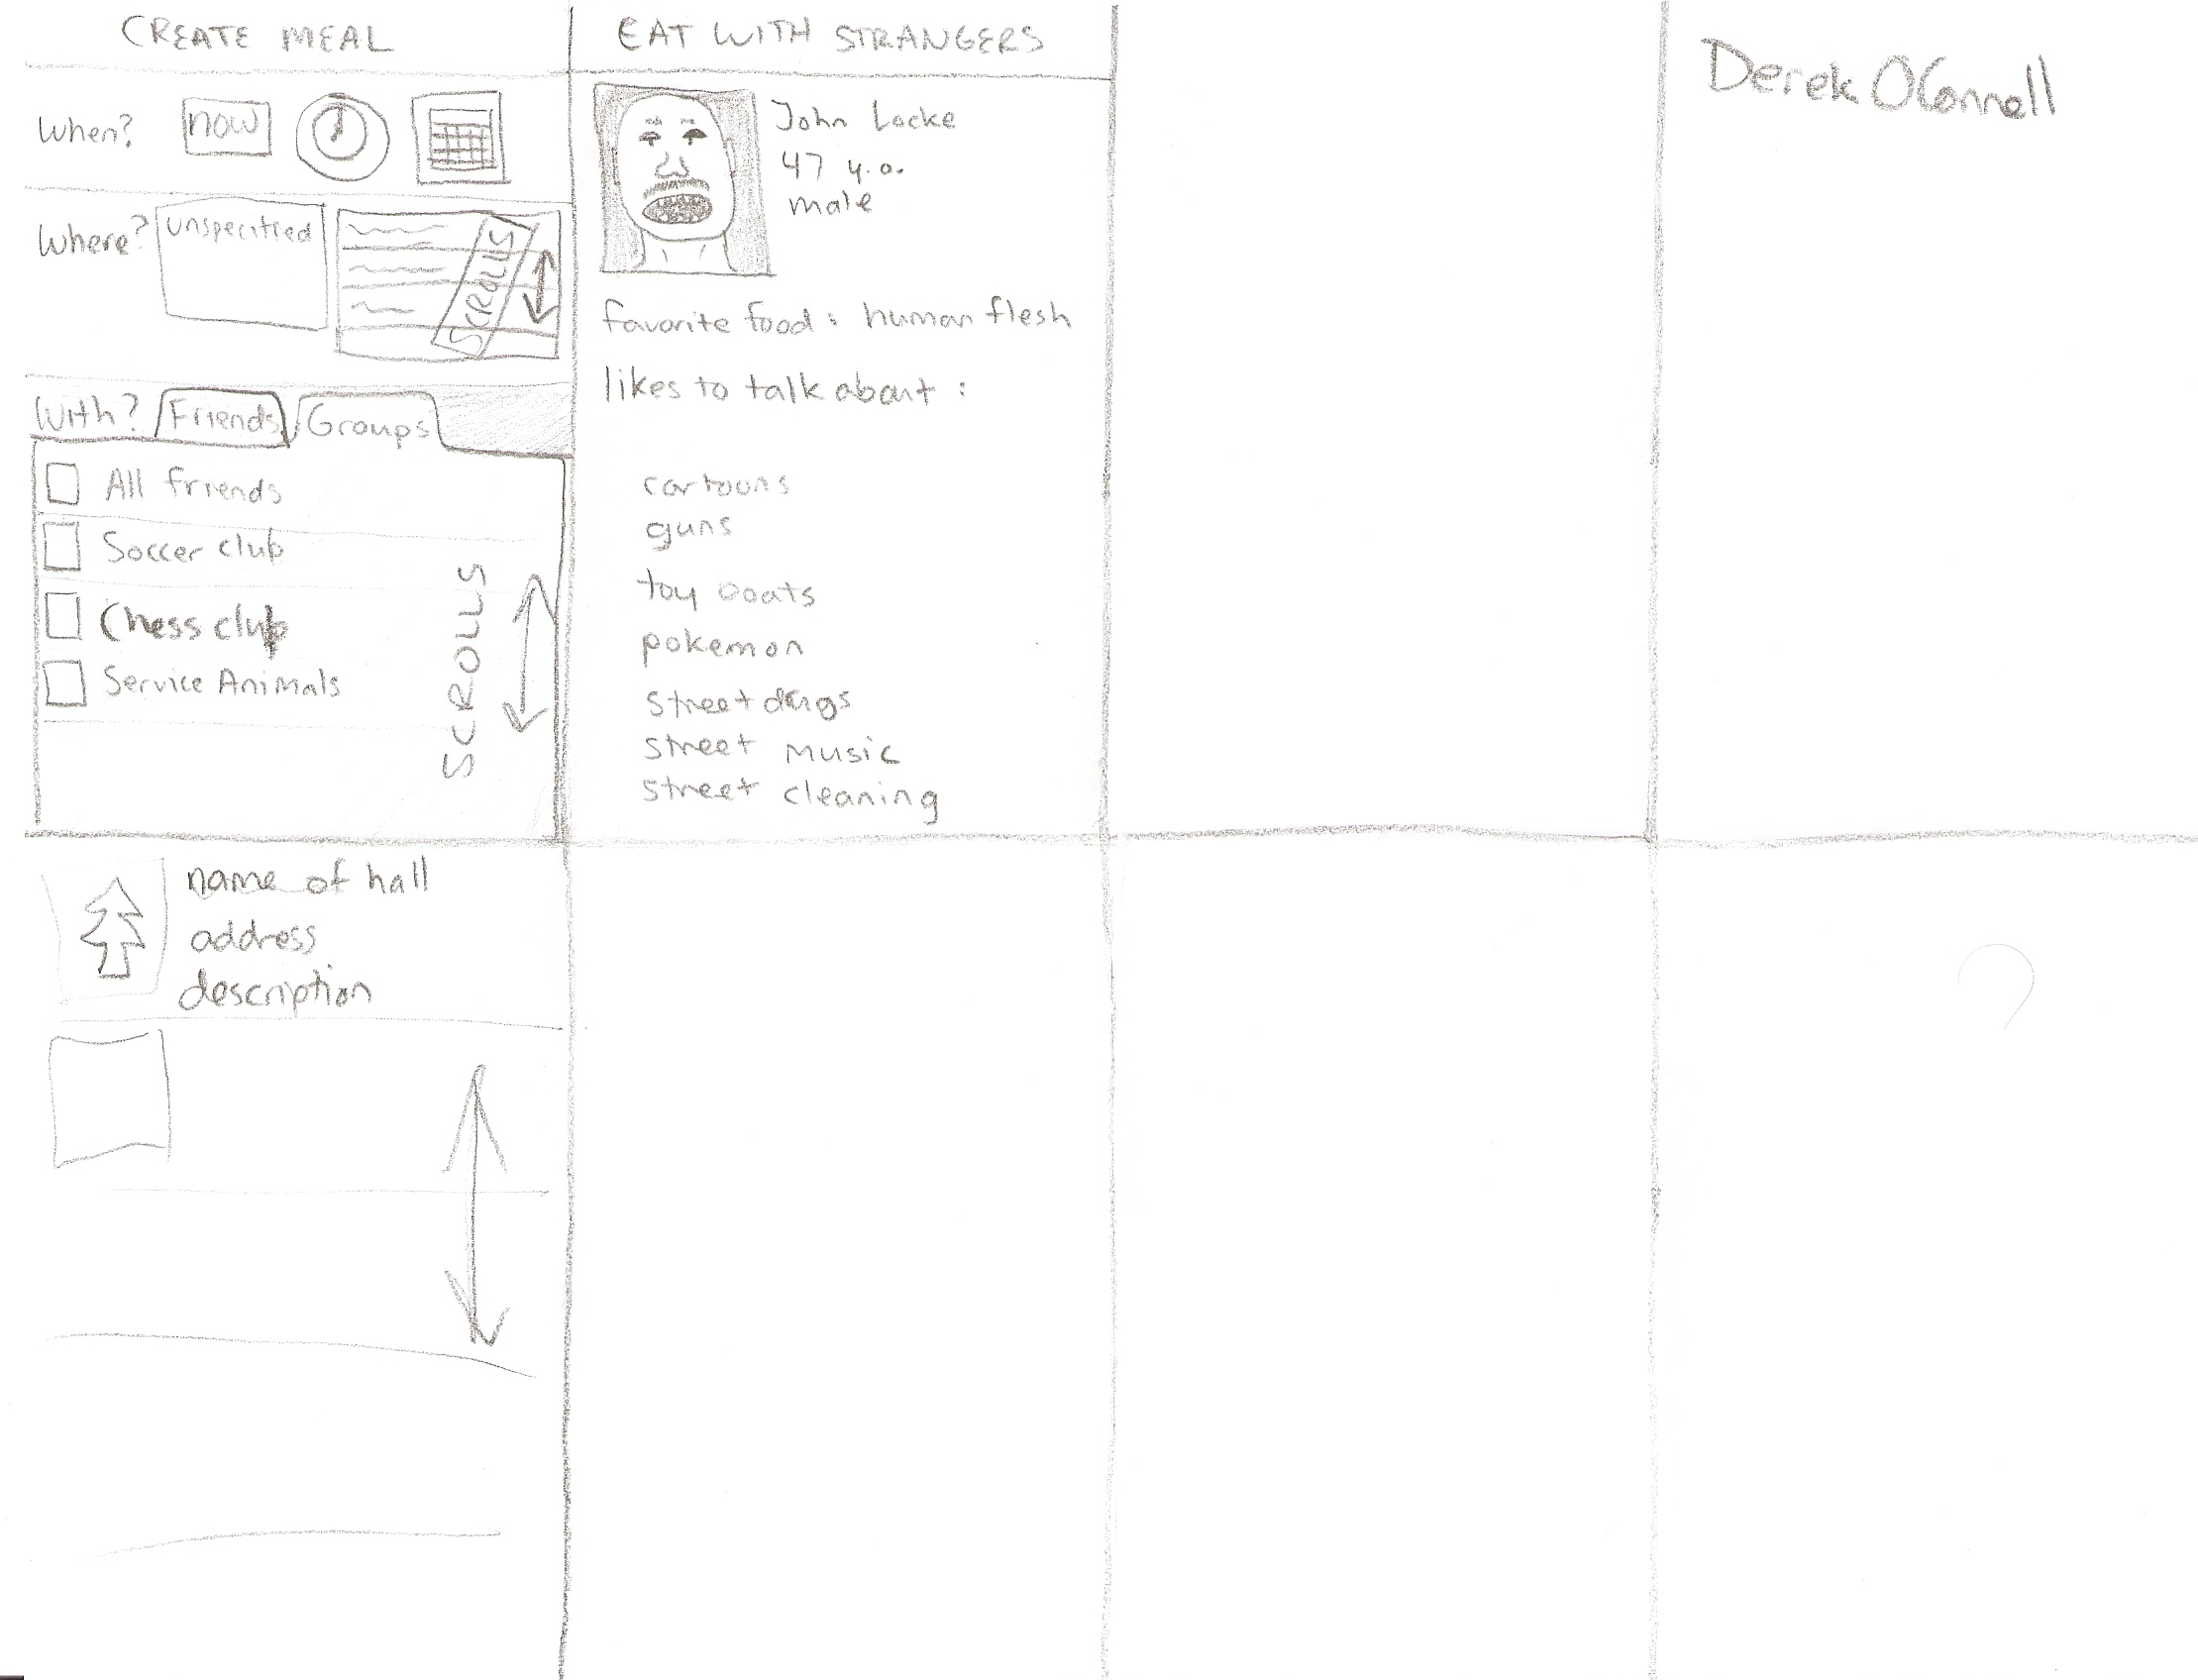
\includegraphics[width=0.8\linewidth]{derek2.jpg}}
\caption{6 Ideas from Derek (cont.)}
\end{figure}

\begin{figure}[h!]
\centering
\fbox{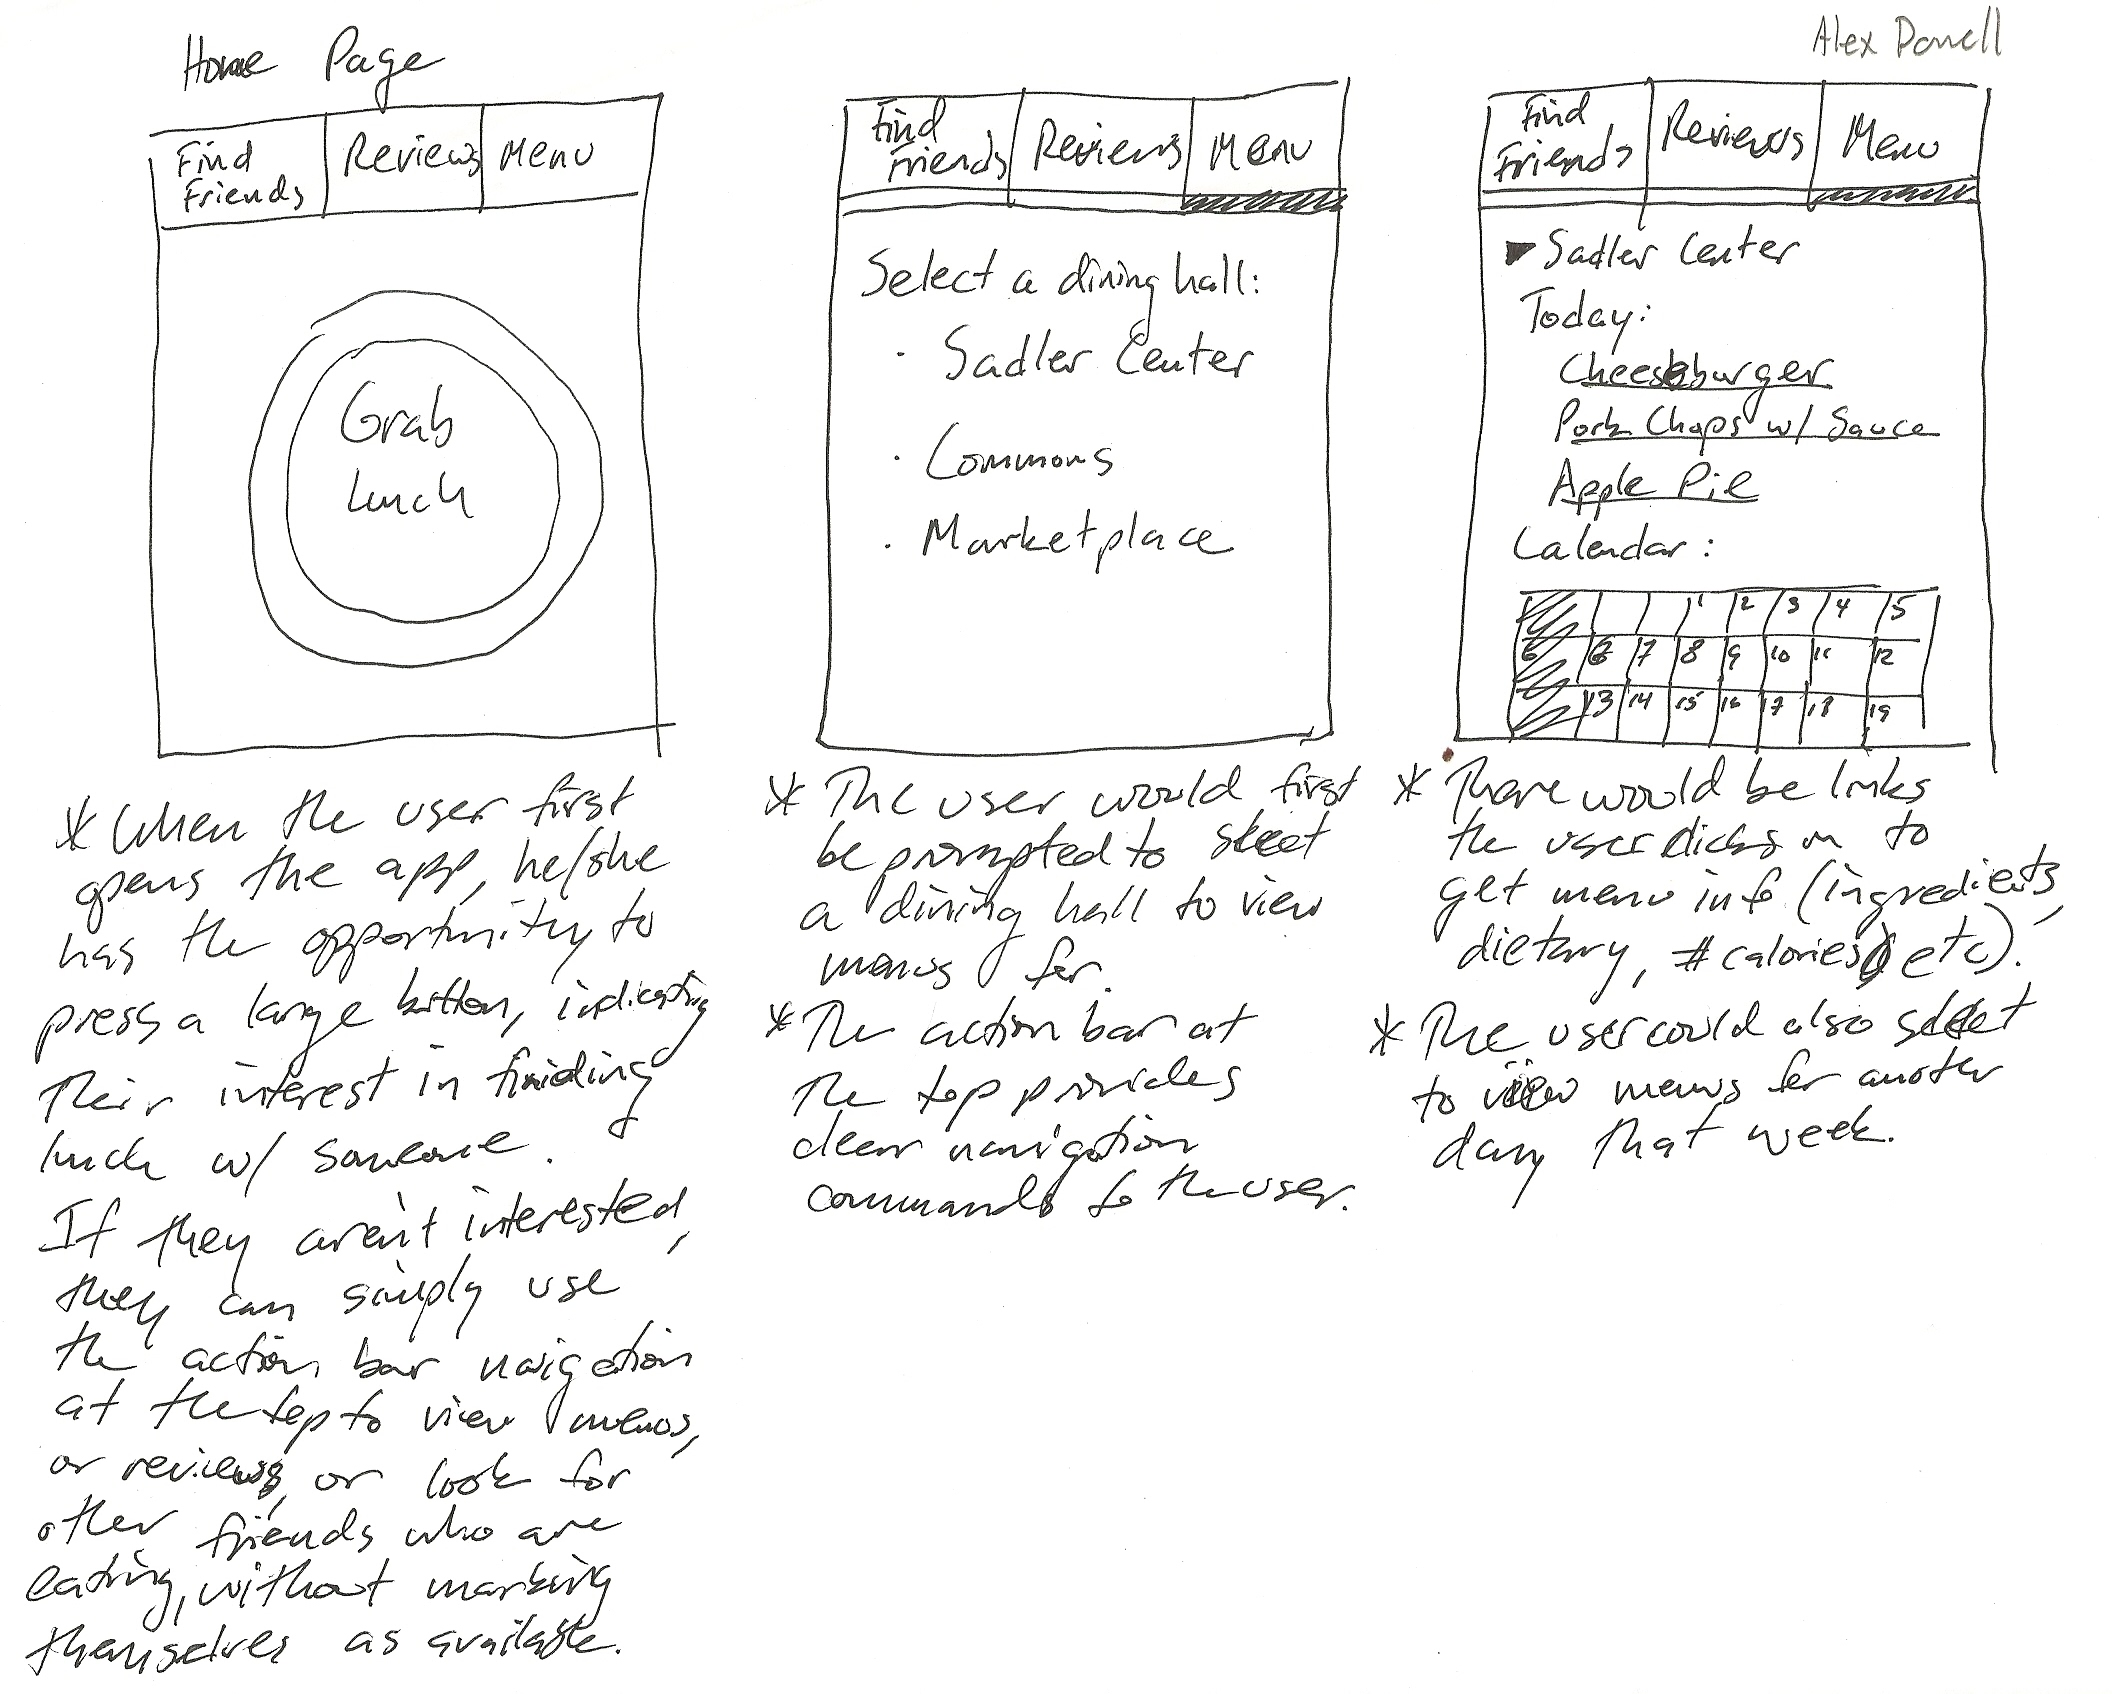
\includegraphics[width=0.8\linewidth]{alex1.jpg}}
\caption{6 Ideas from Alex}
\end{figure}

\begin{figure}[h!]
\centering
\fbox{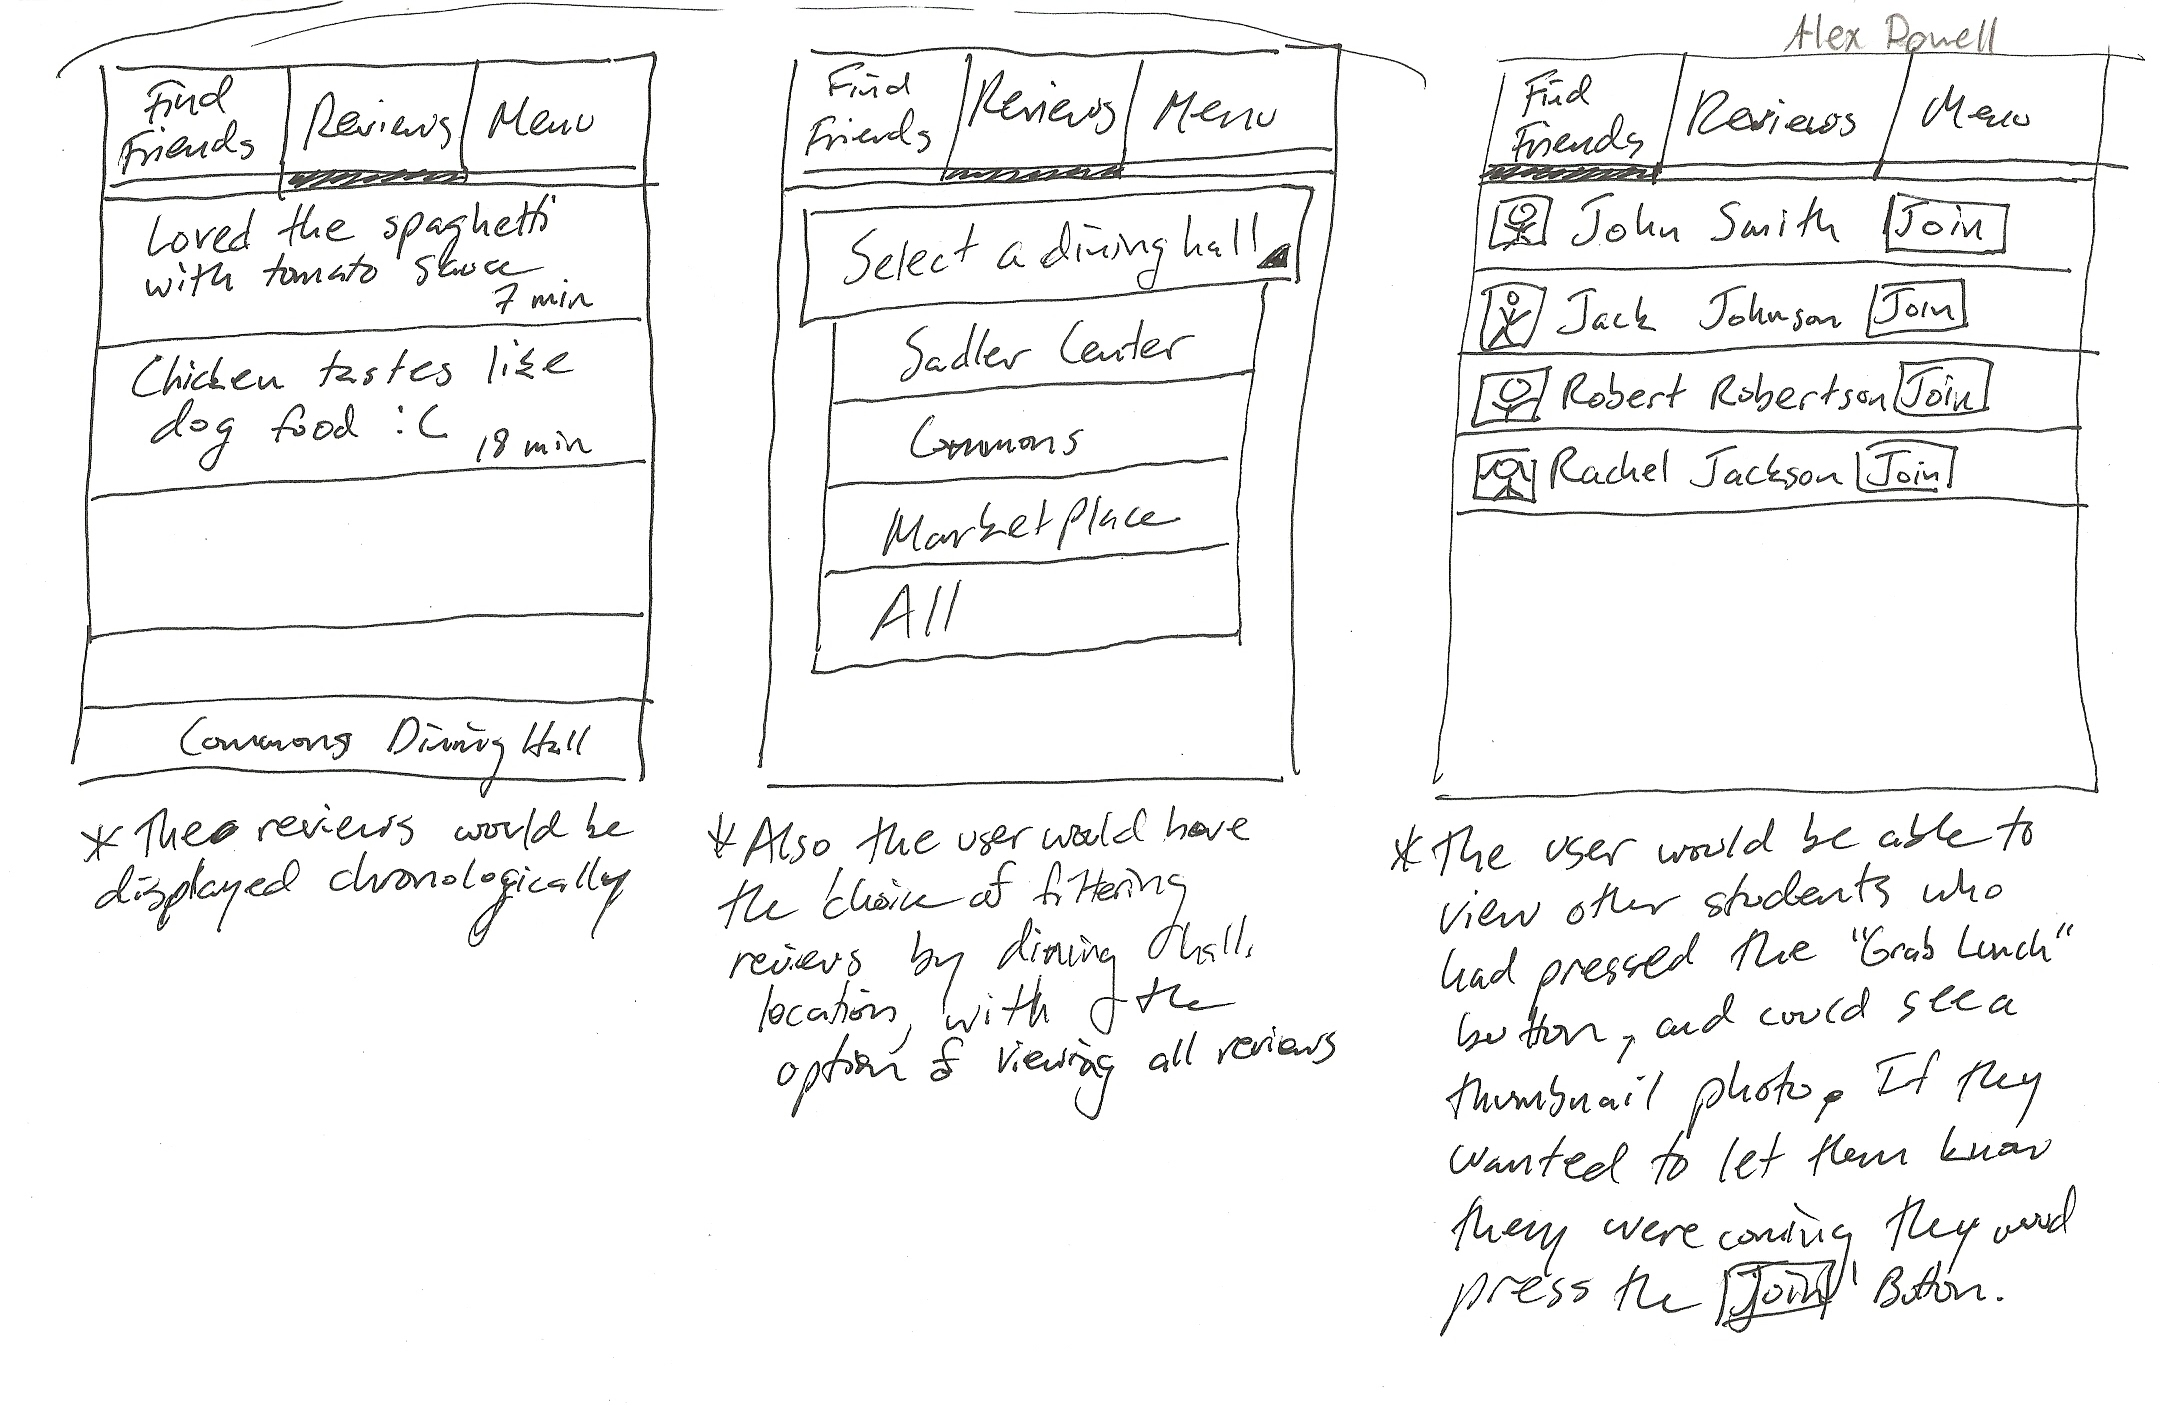
\includegraphics[width=0.8\linewidth]{alex2.jpg}}
\caption{6 Ideas from Alex (cont.)}
\end{figure}

\begin{figure}[h!]
\centering
\fbox{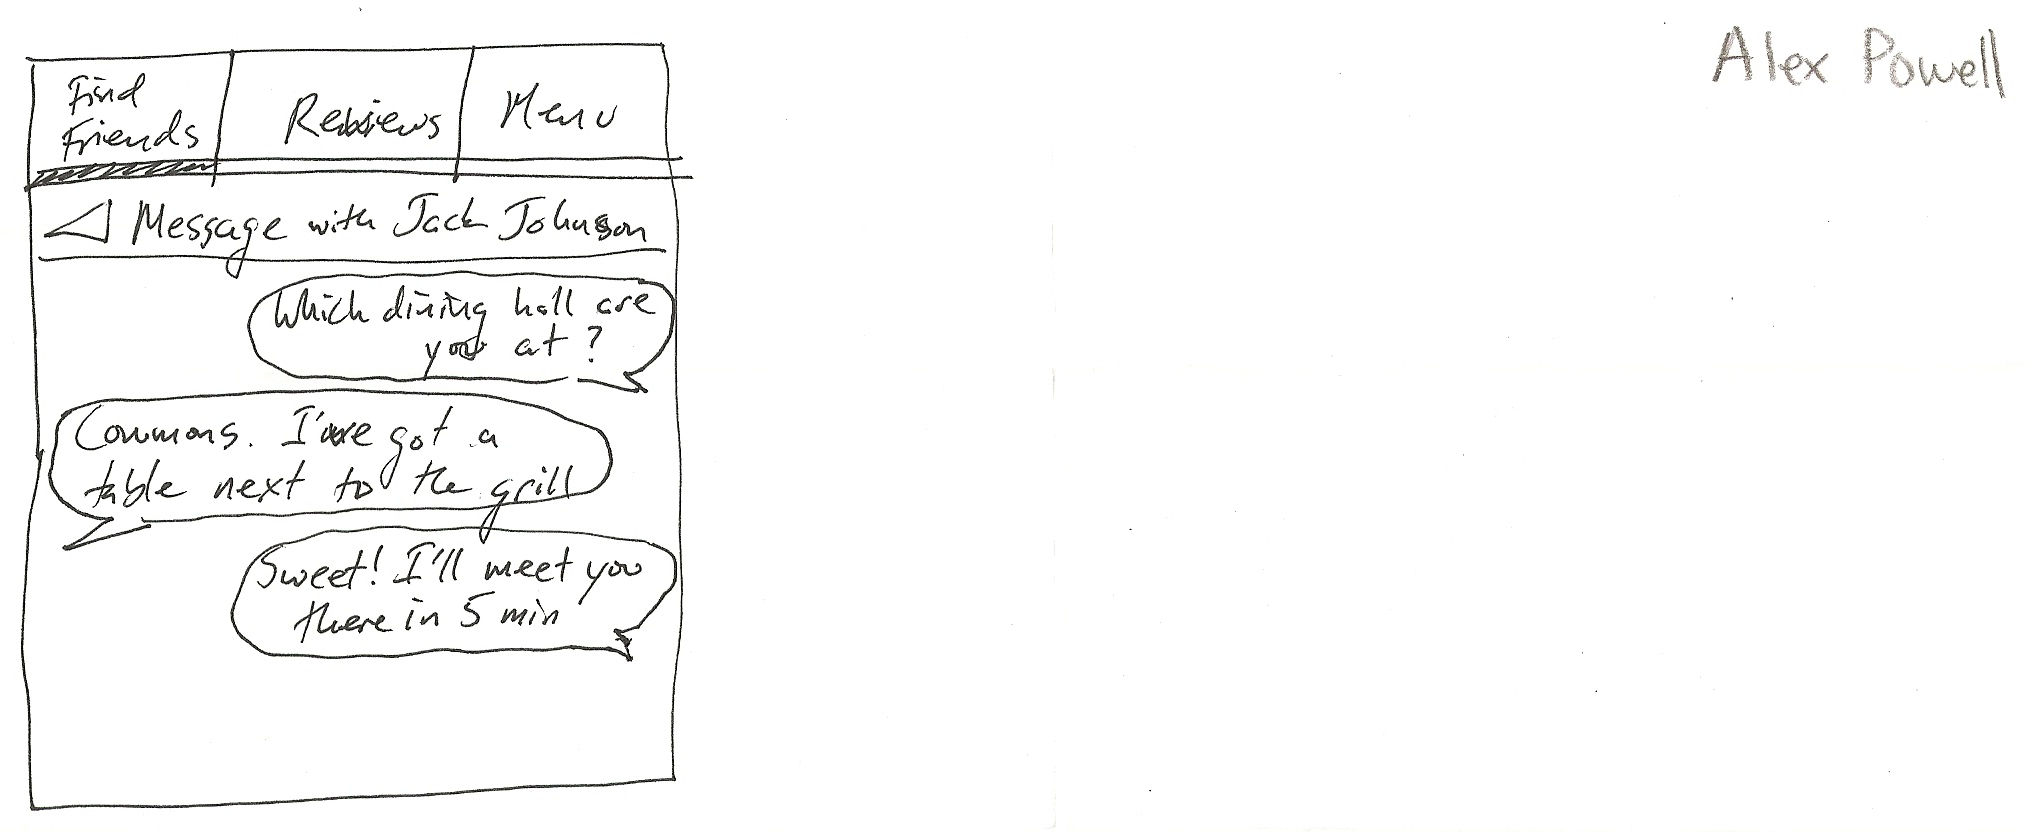
\includegraphics[width=0.8\linewidth]{alex3.jpg}}
\caption{6 Ideas from Alex (cont.)}
\end{figure}

\begin{figure}[h!]
\centering
\fbox{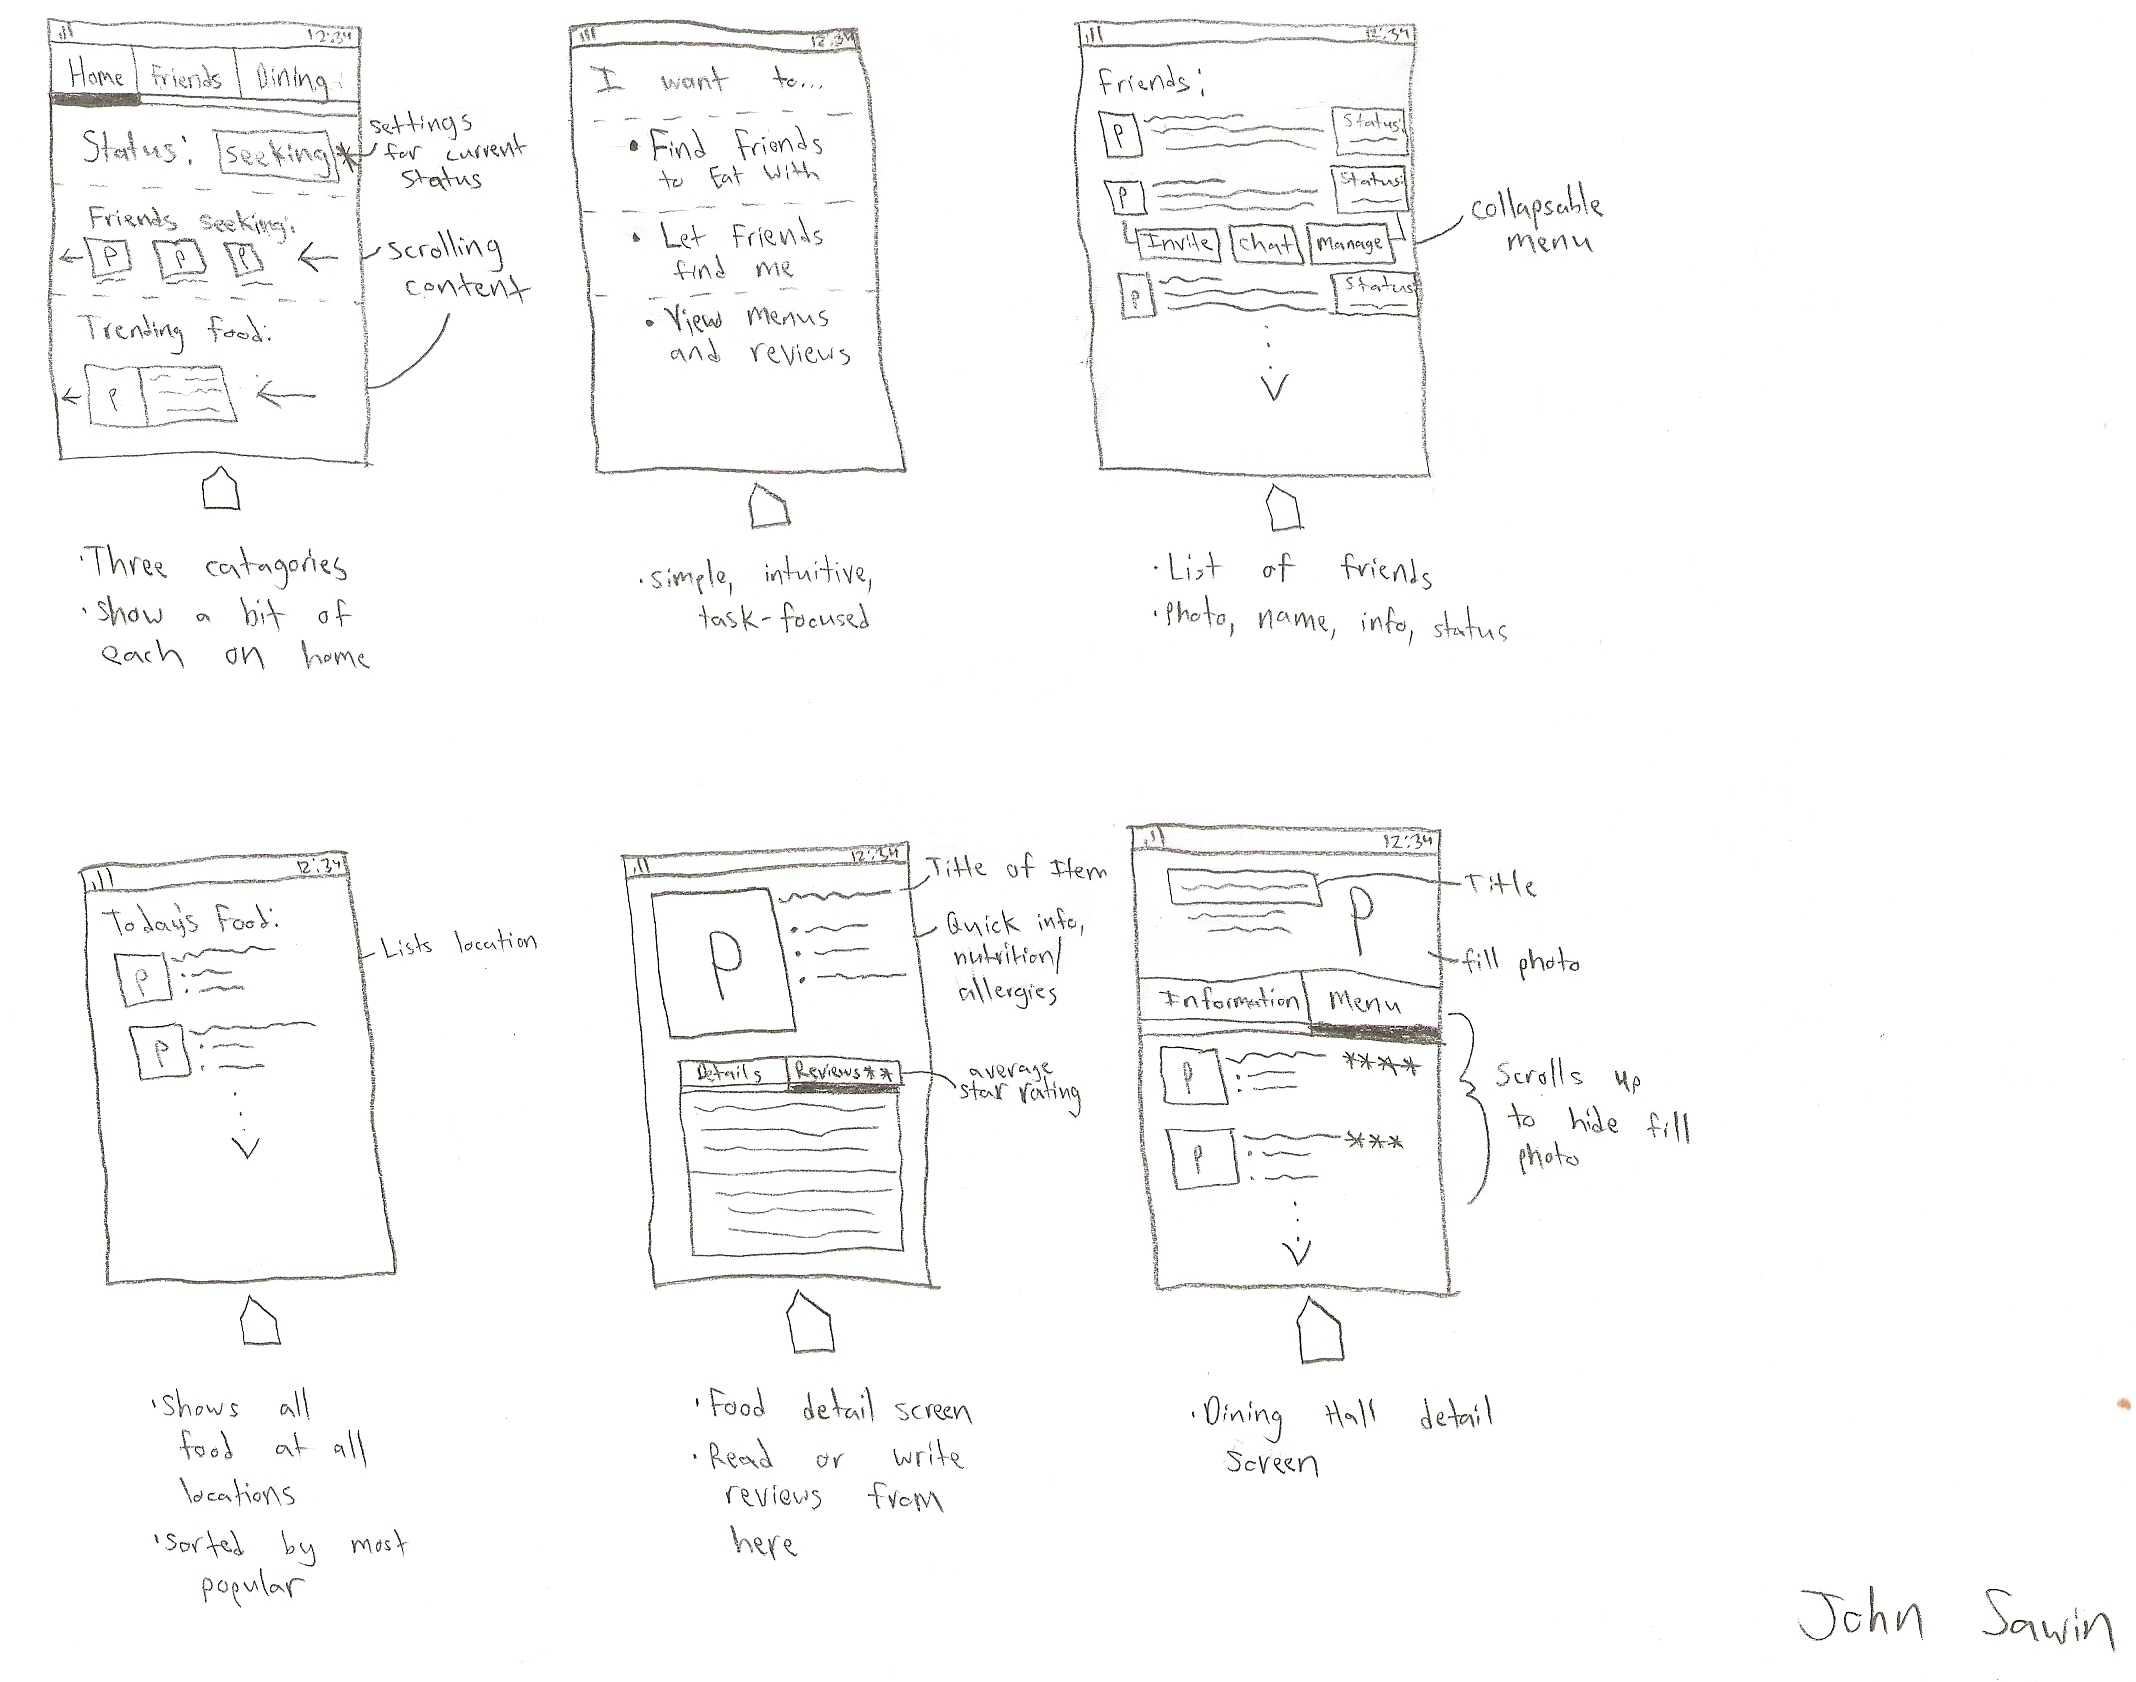
\includegraphics[width=0.8\linewidth]{john.jpg}}
\caption{6 Ideas from John}
\end{figure}

\begin{figure}[h!]
\centering
\fbox{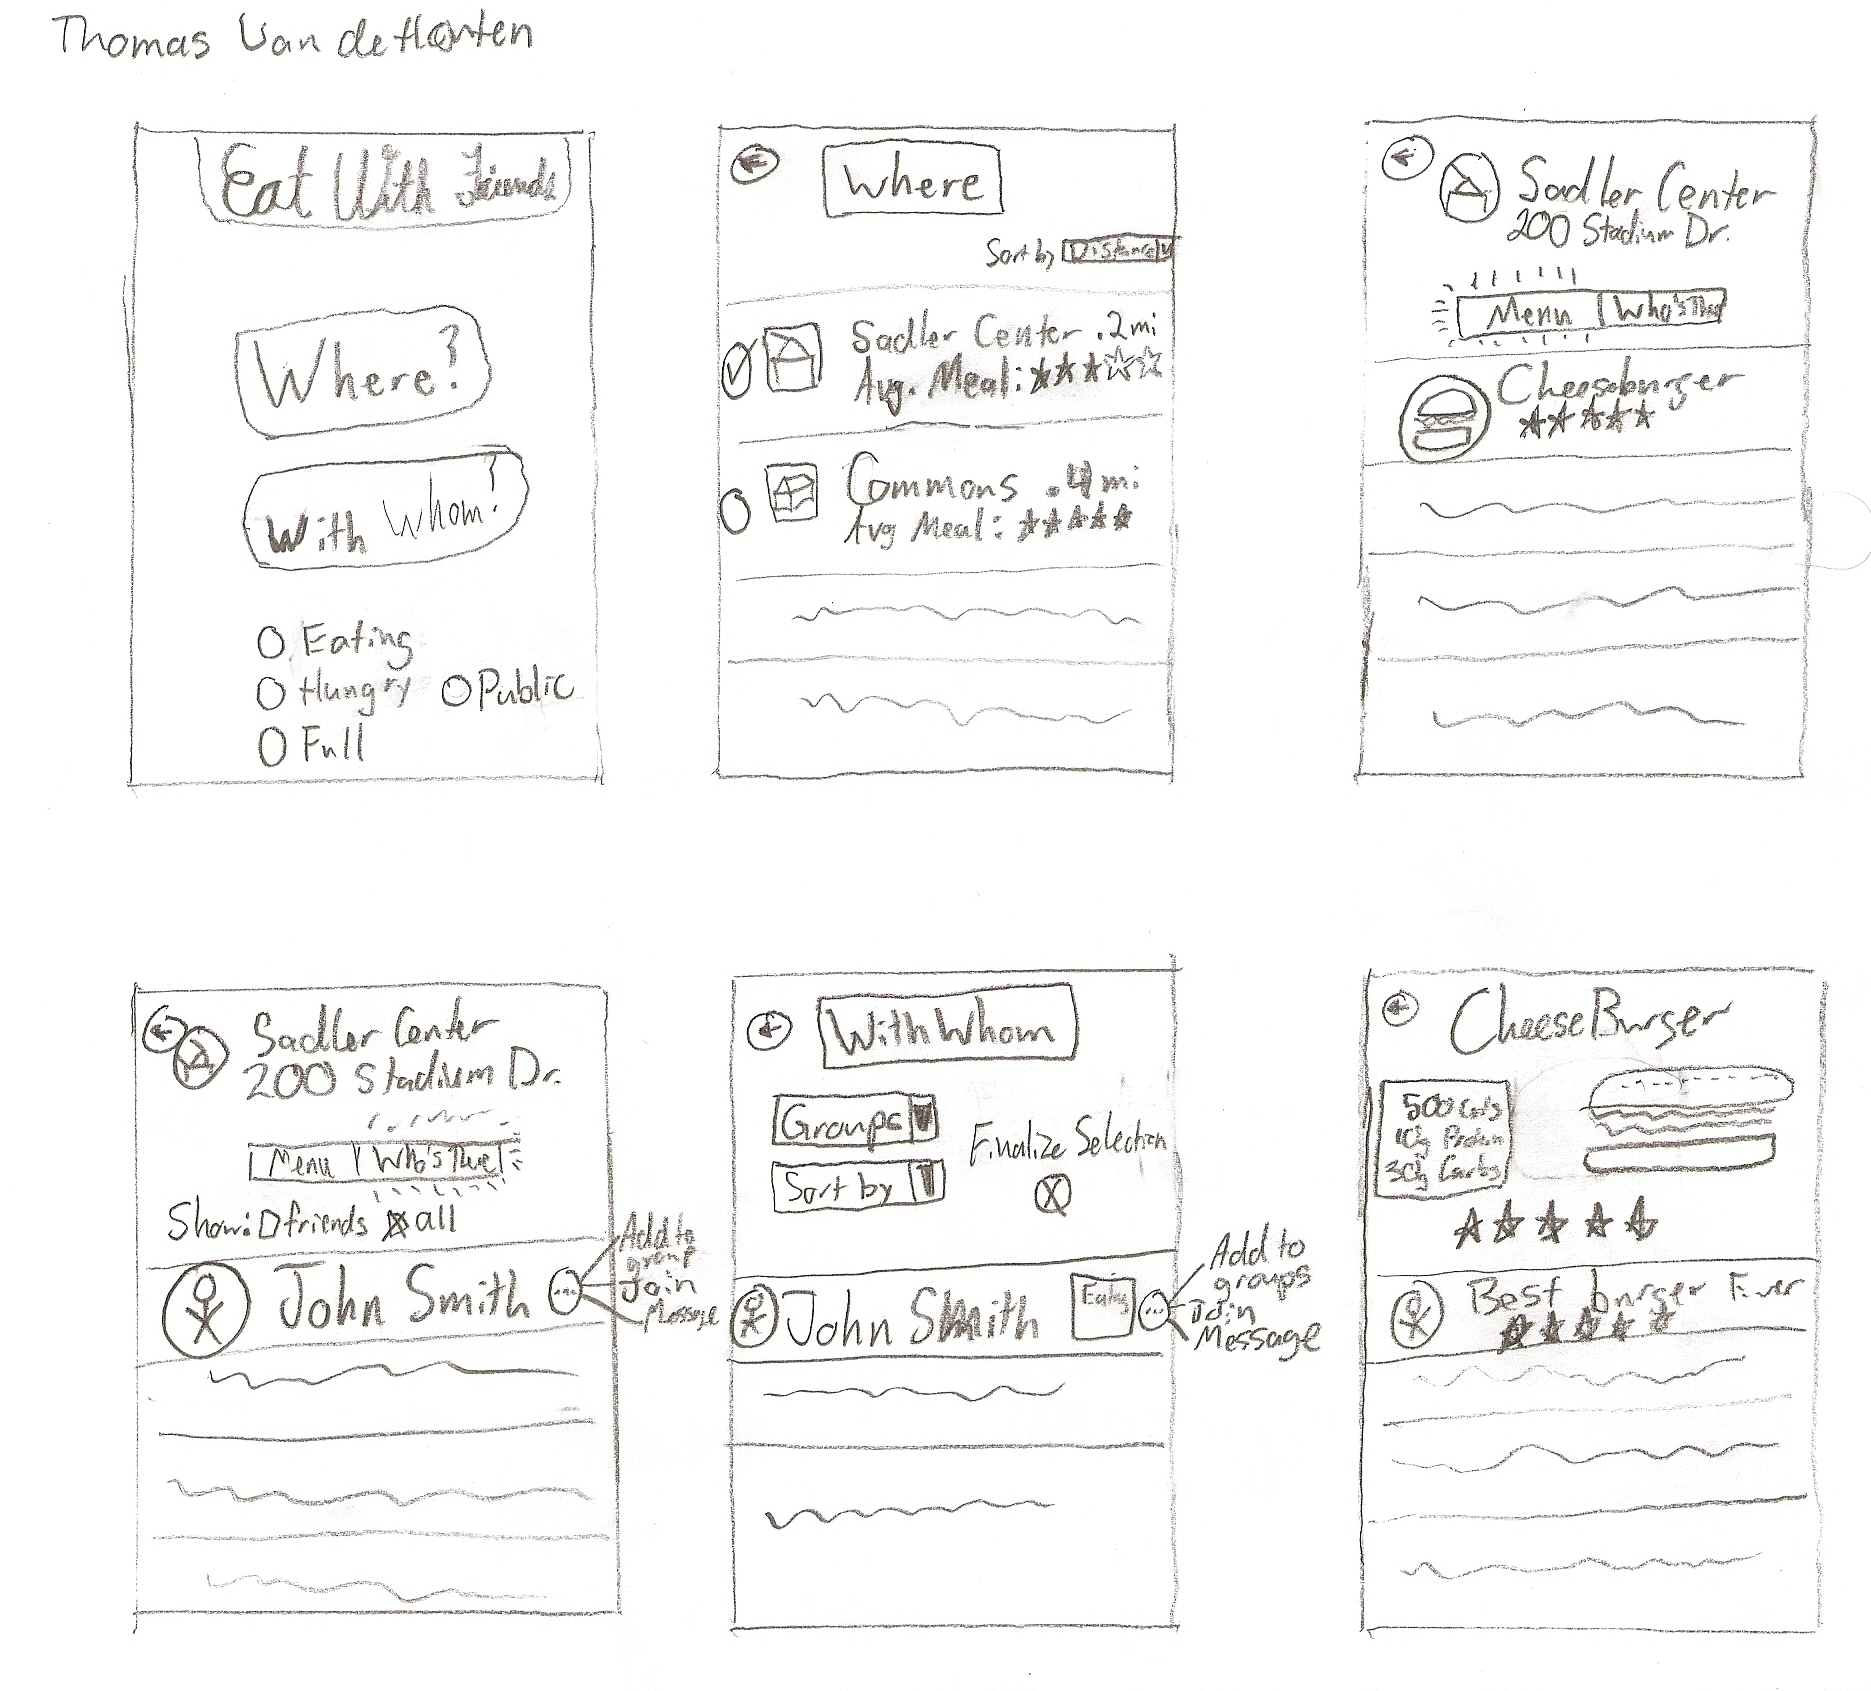
\includegraphics[width=0.8\linewidth]{thomas.jpg}}
\caption{6 Ideas from Thomas}
\end{figure}

\clearpage
\section{Our Best Design}

\begin{figure}[h!]
\centering
\fbox{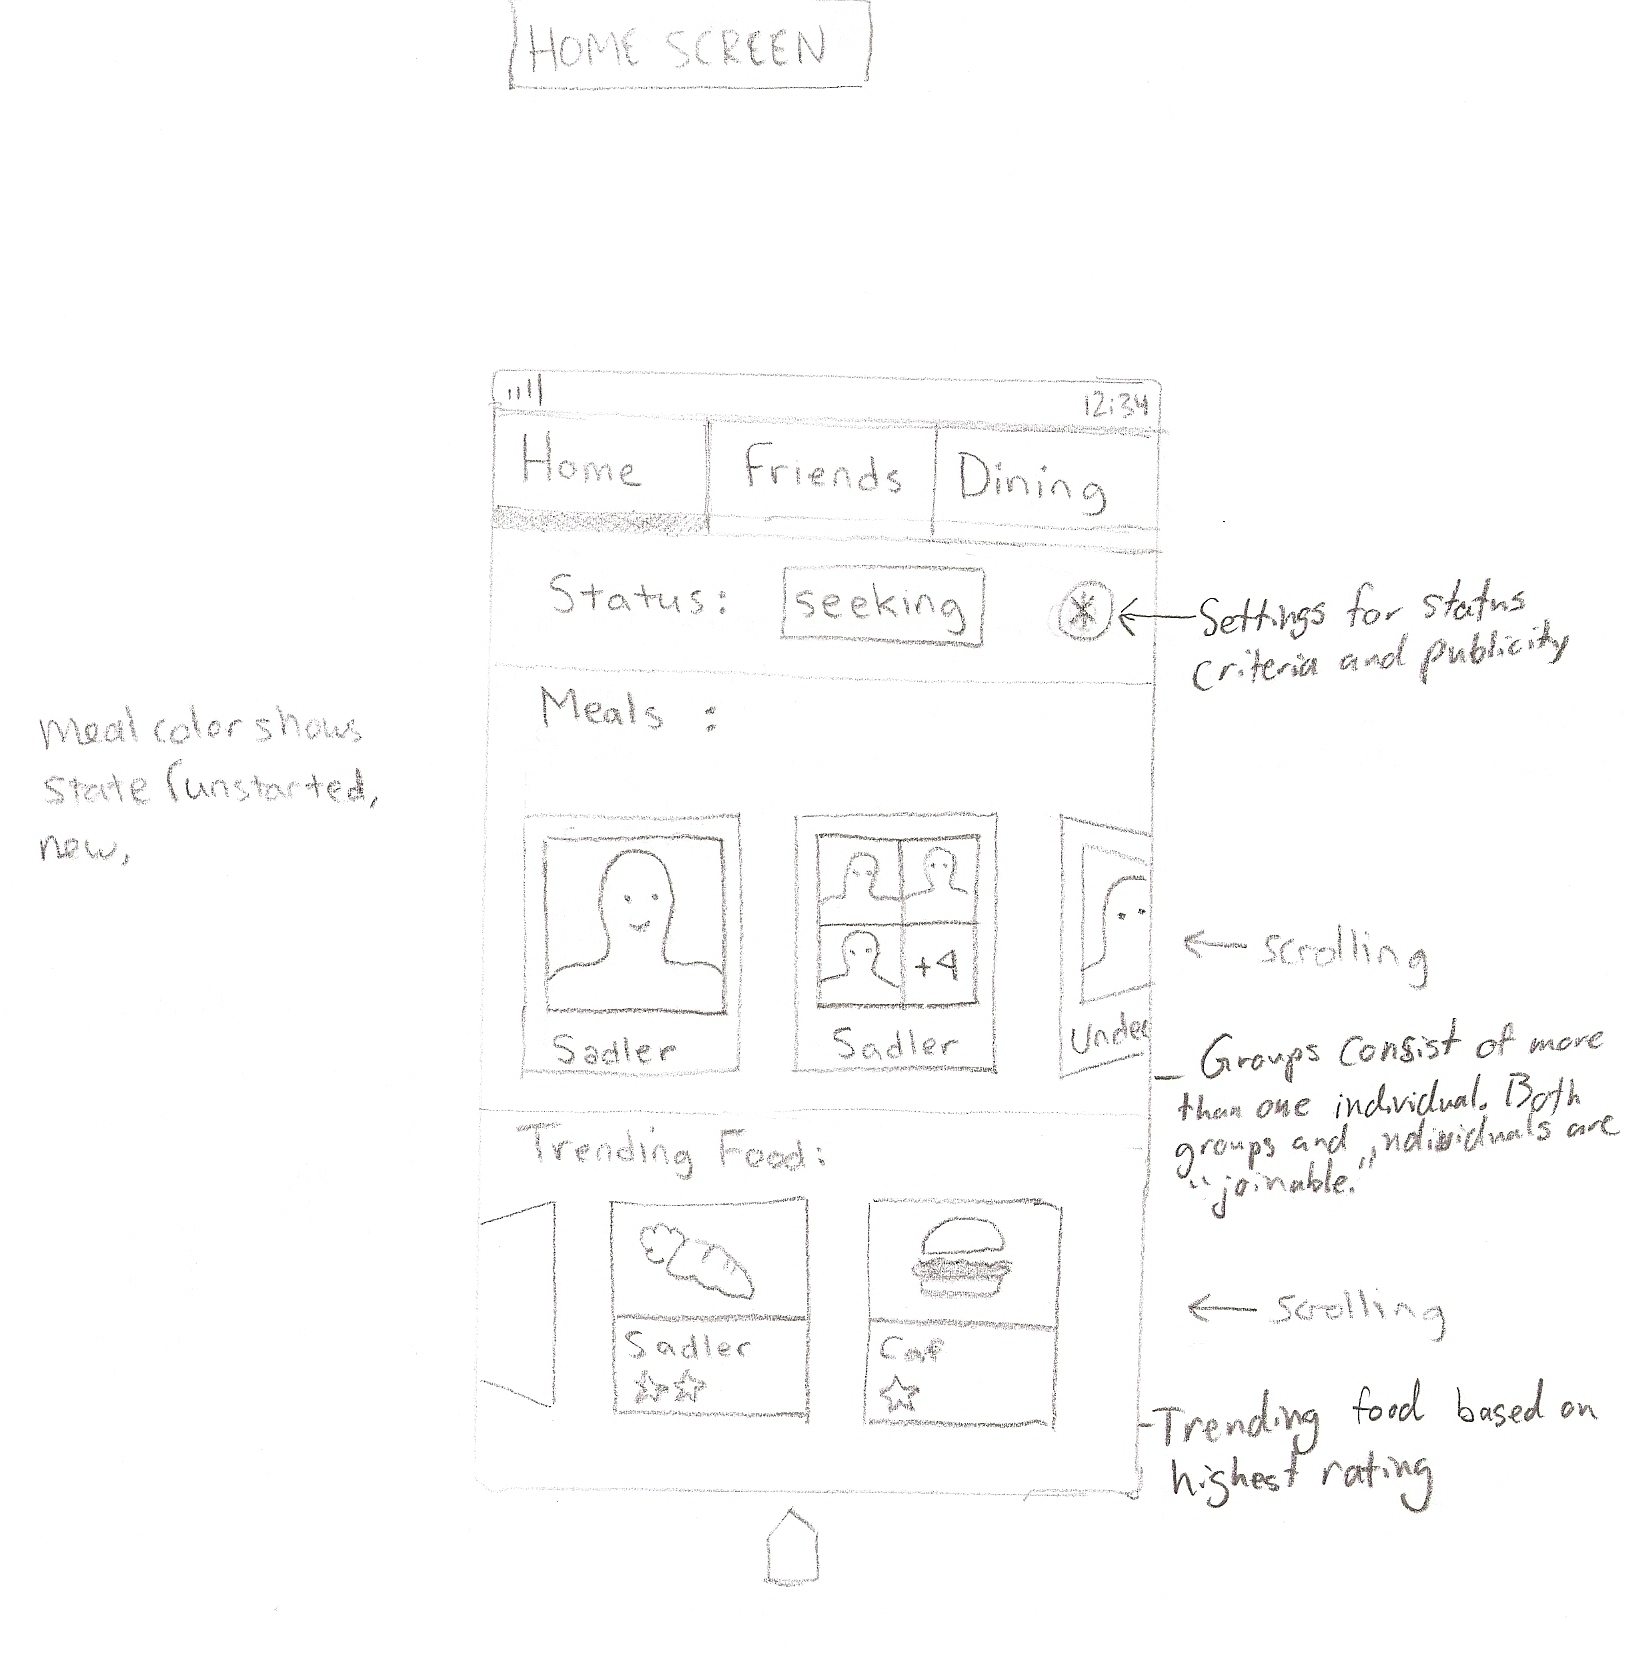
\includegraphics[width=0.8\linewidth]{team1.jpg}}
\caption{Home screen}
\end{figure}

\begin{figure}[h!]
\centering
\fbox{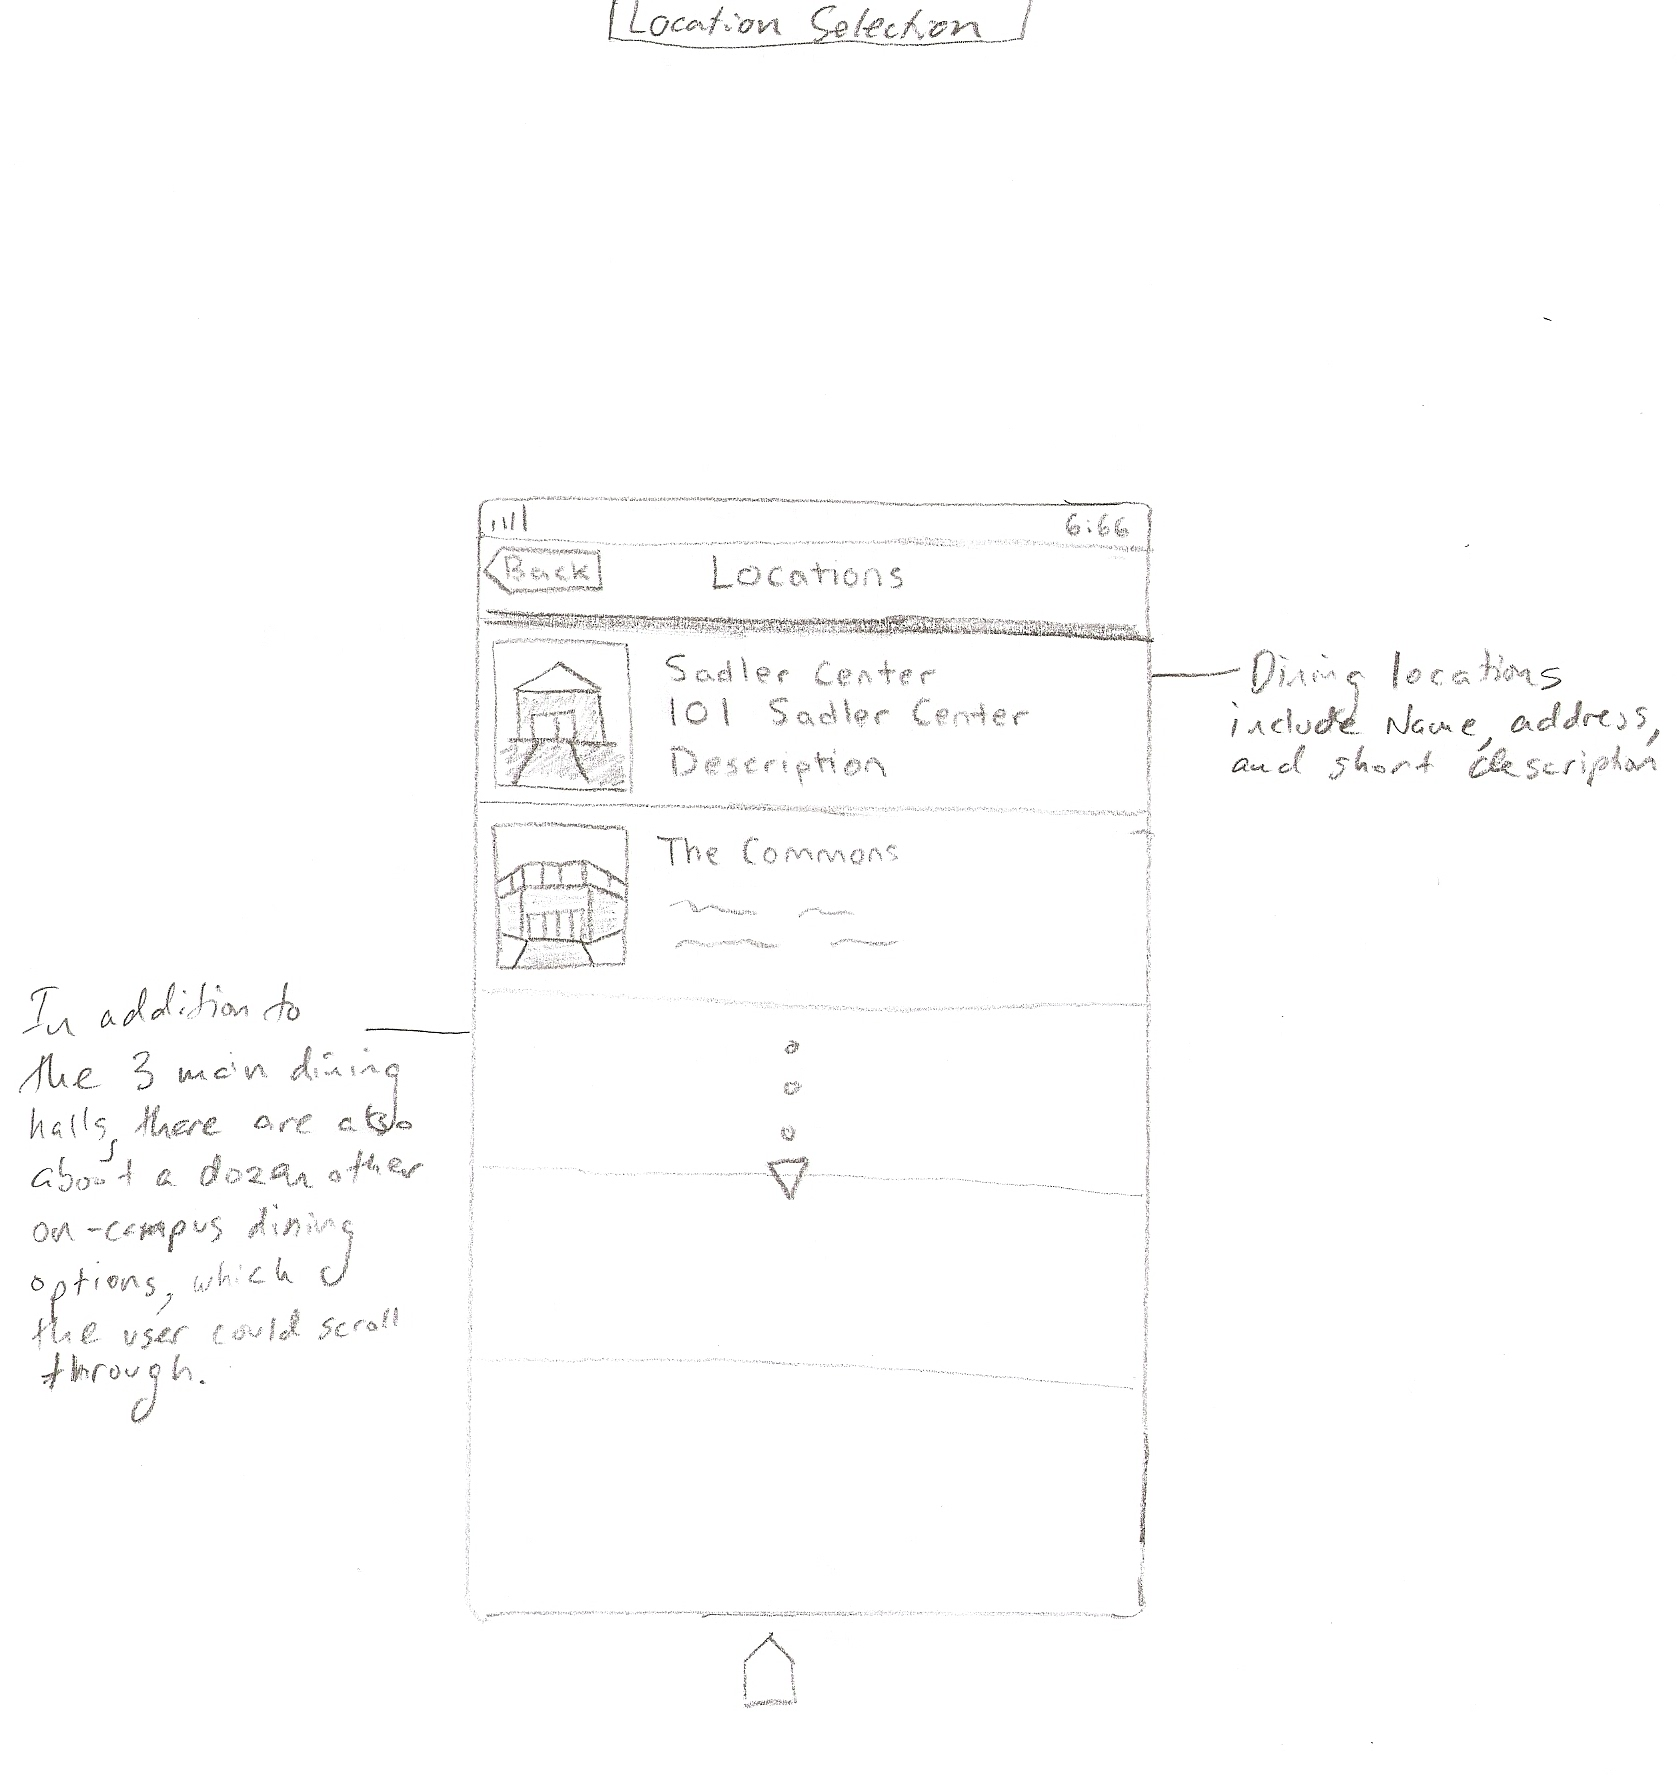
\includegraphics[width=0.8\linewidth]{team2.jpg}}
\caption{Location Selection Page}
\end{figure}

\begin{figure}[h!]
\centering
\fbox{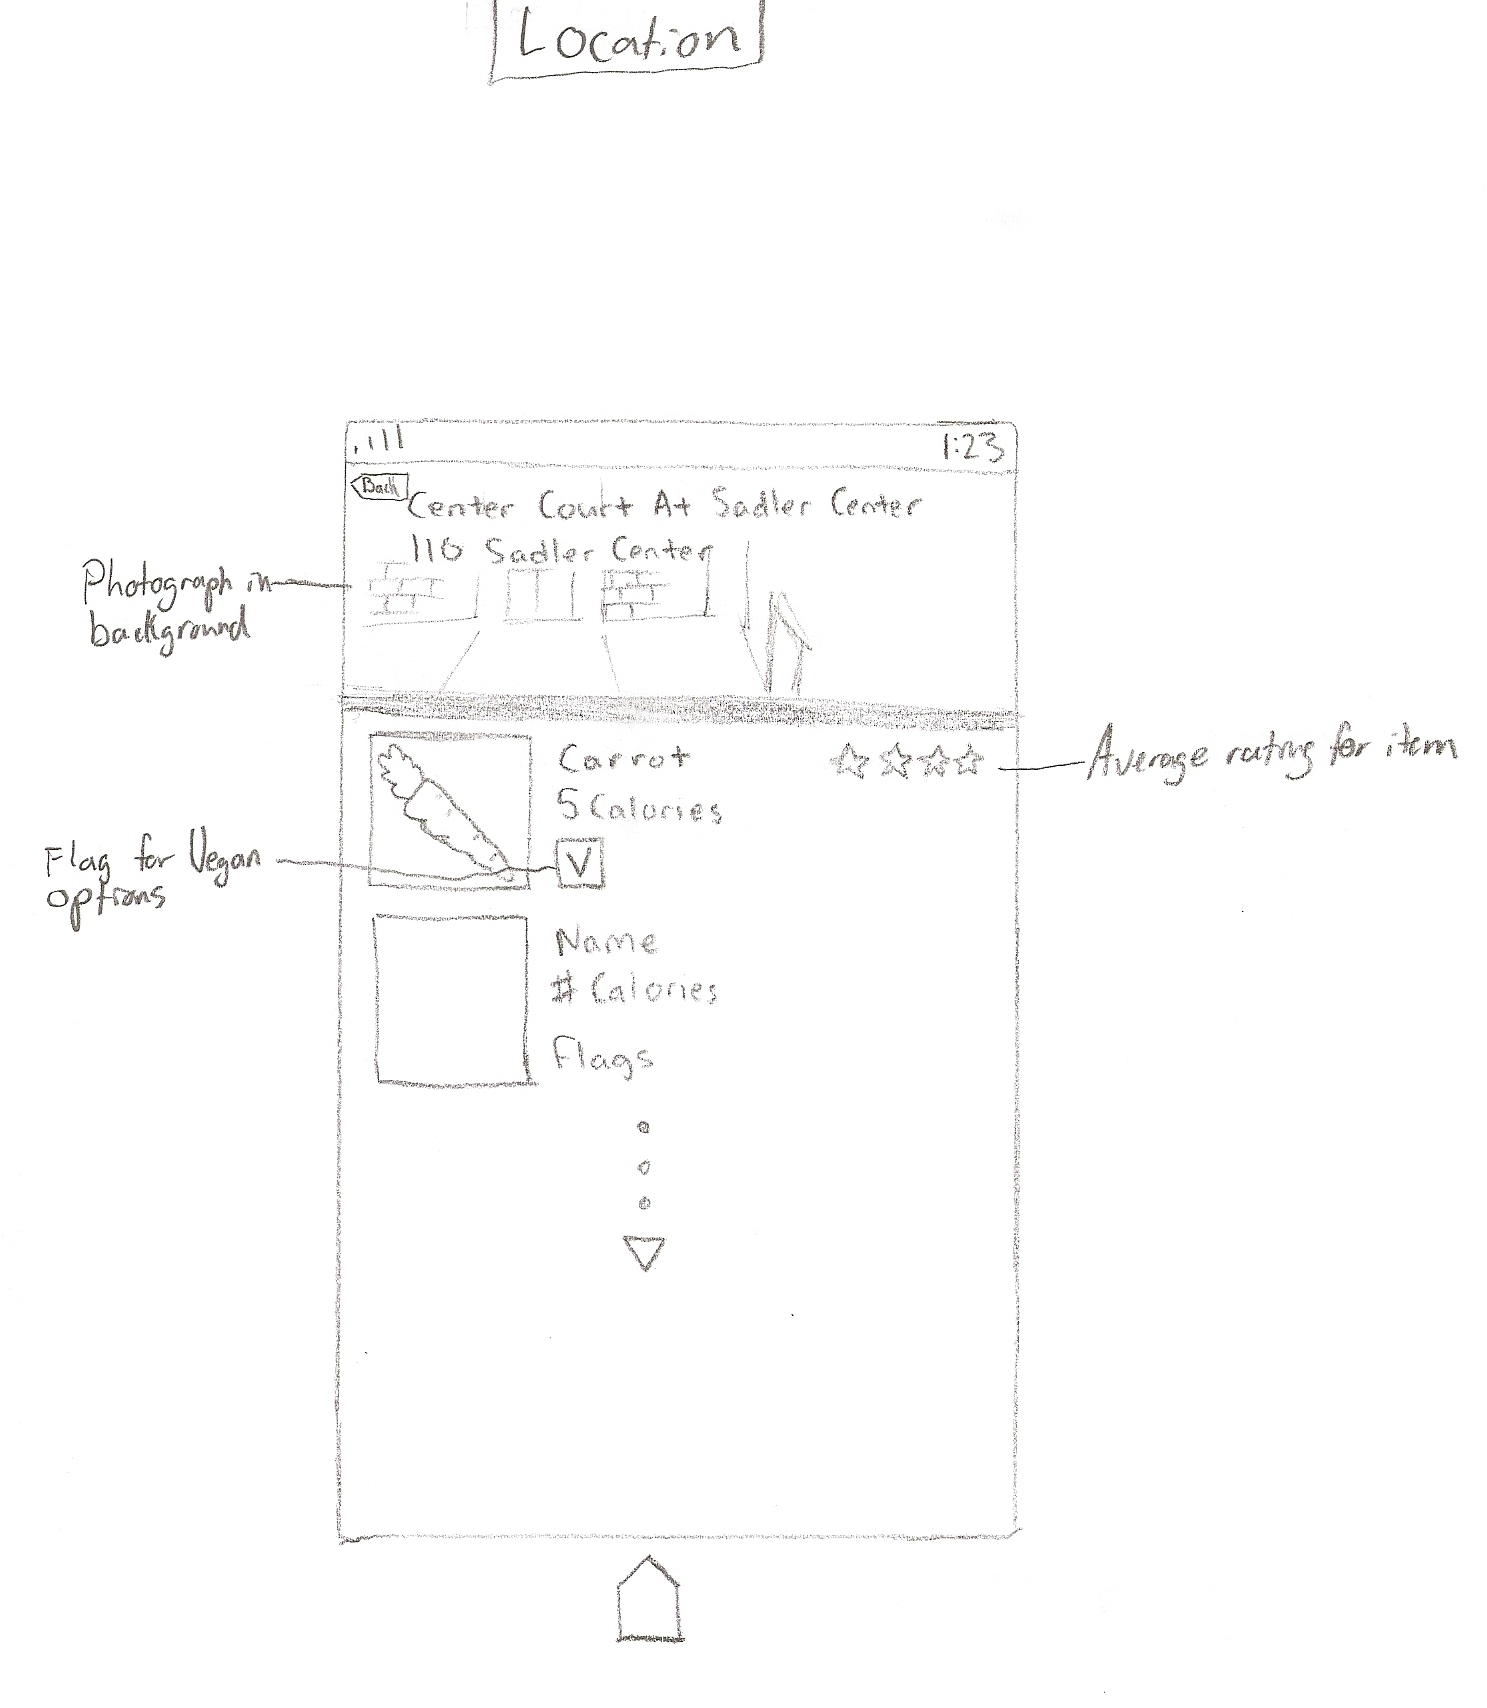
\includegraphics[width=0.8\linewidth]{team3.jpg}}
\caption{Location Details Page}
\end{figure}

\begin{figure}[h!]
\centering
\fbox{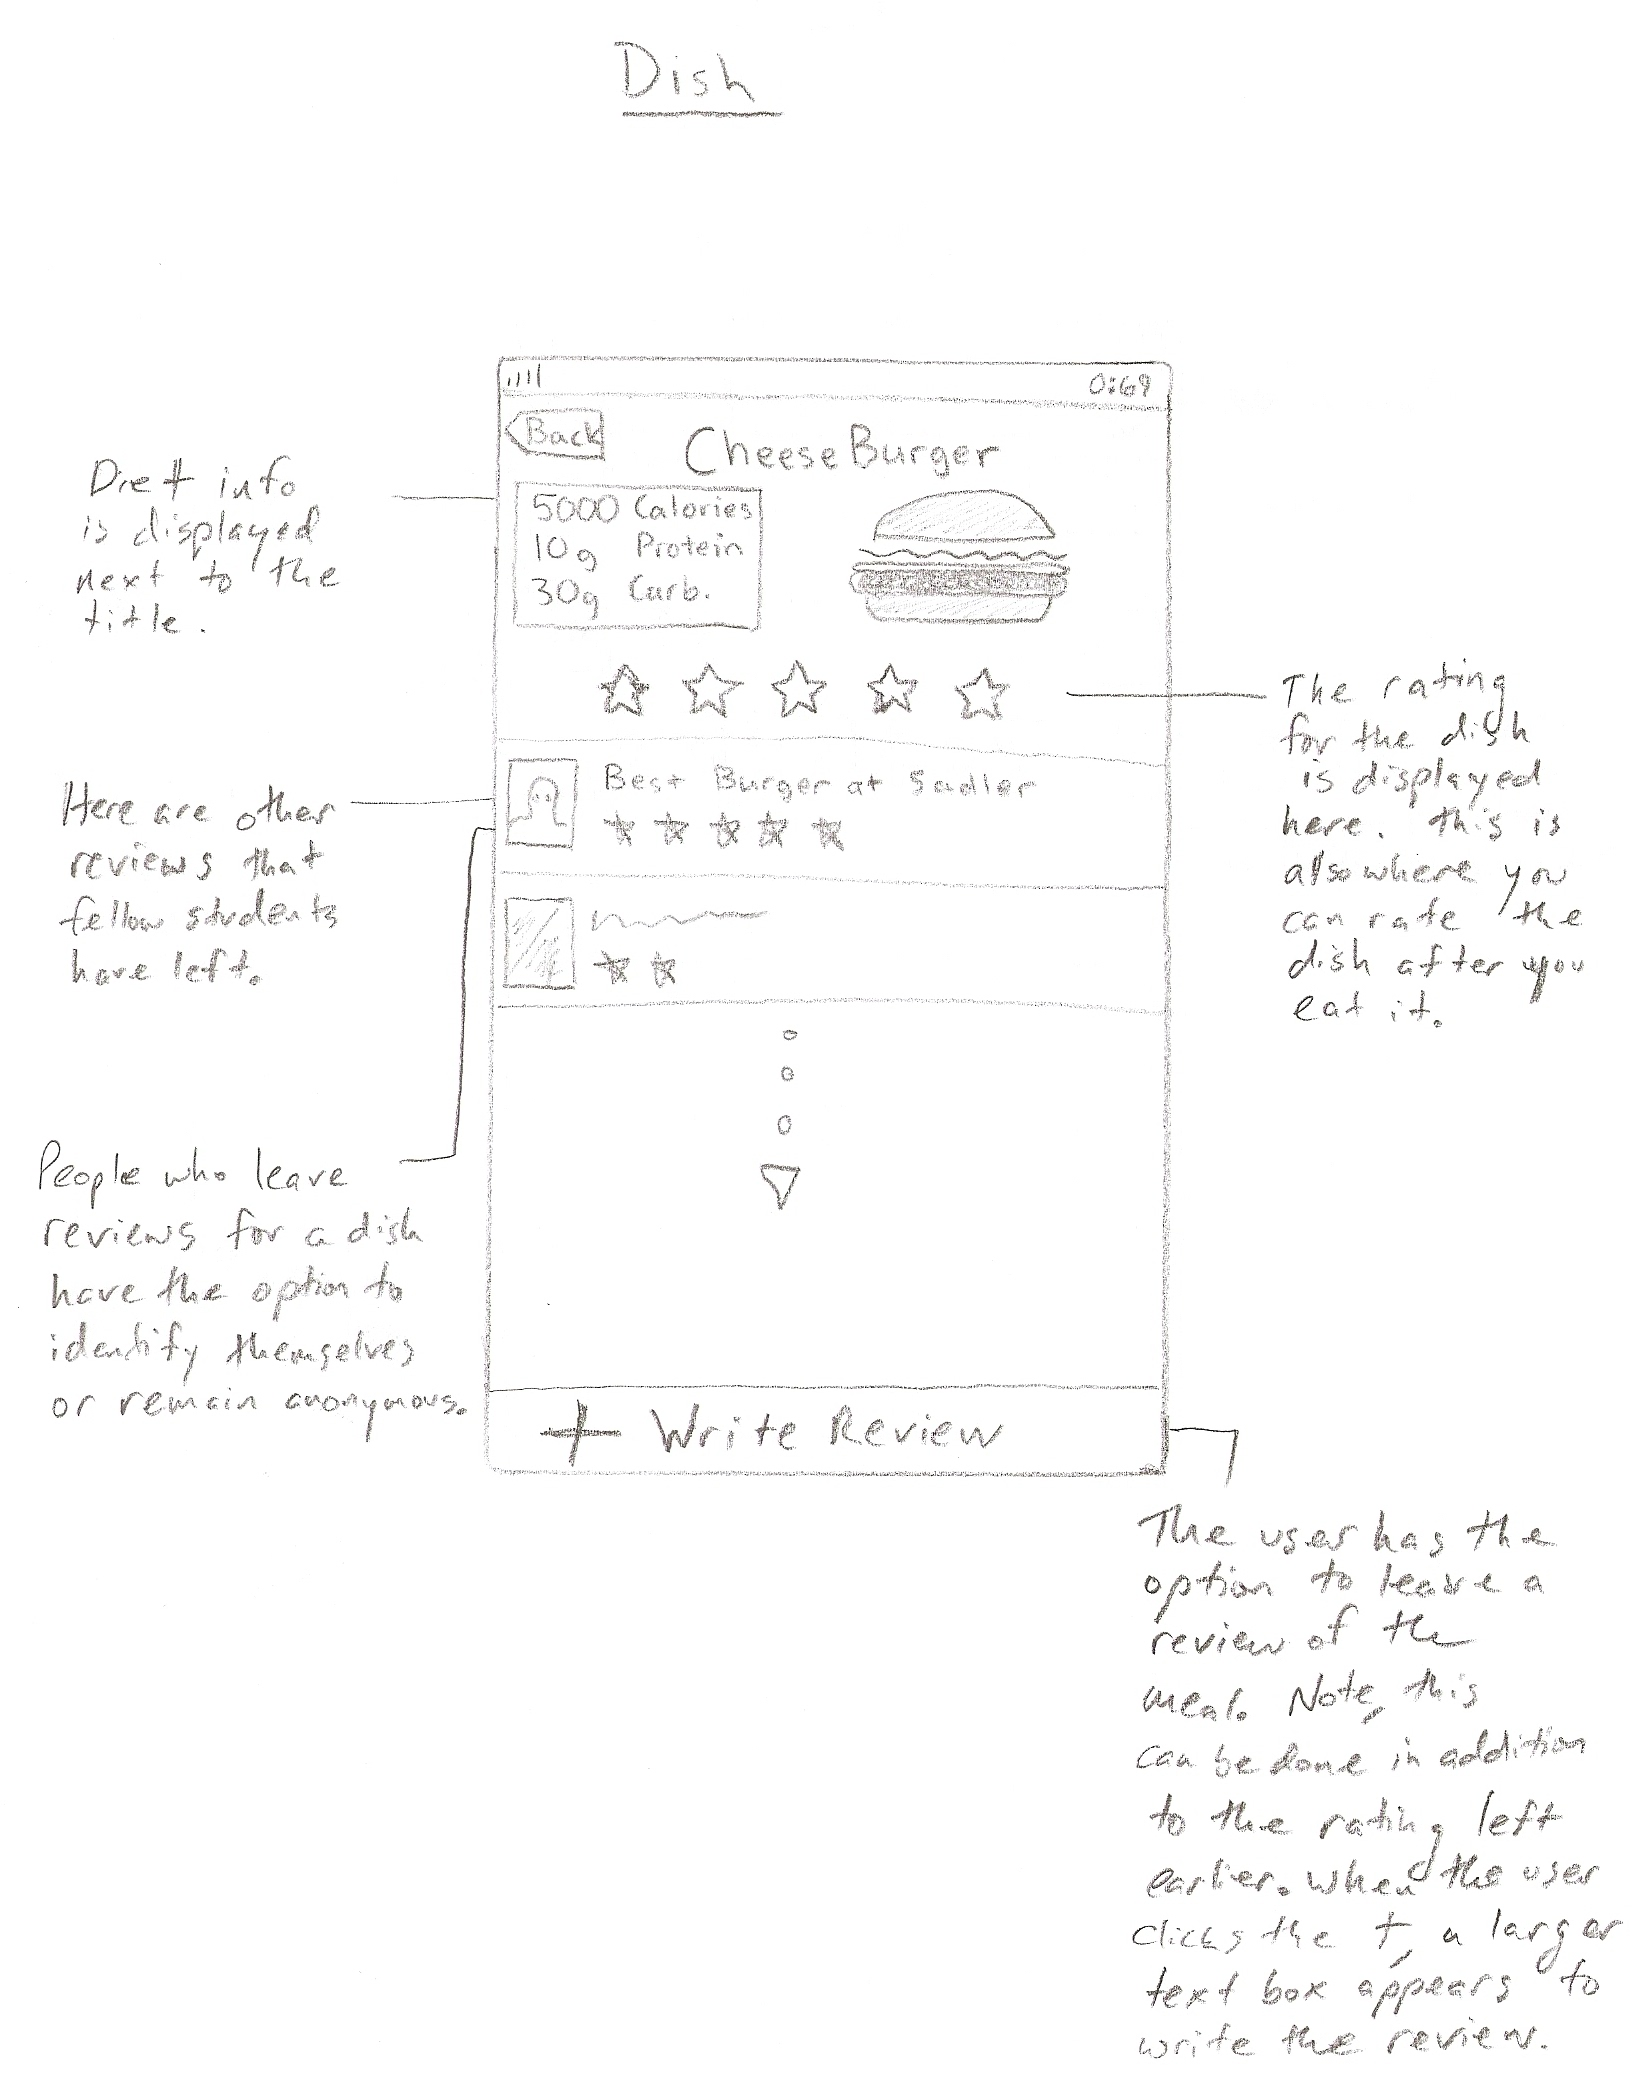
\includegraphics[width=0.8\linewidth]{team4.jpg}}
\caption{Dish Page}
\end{figure}

\begin{figure}[h!]
\centering
\fbox{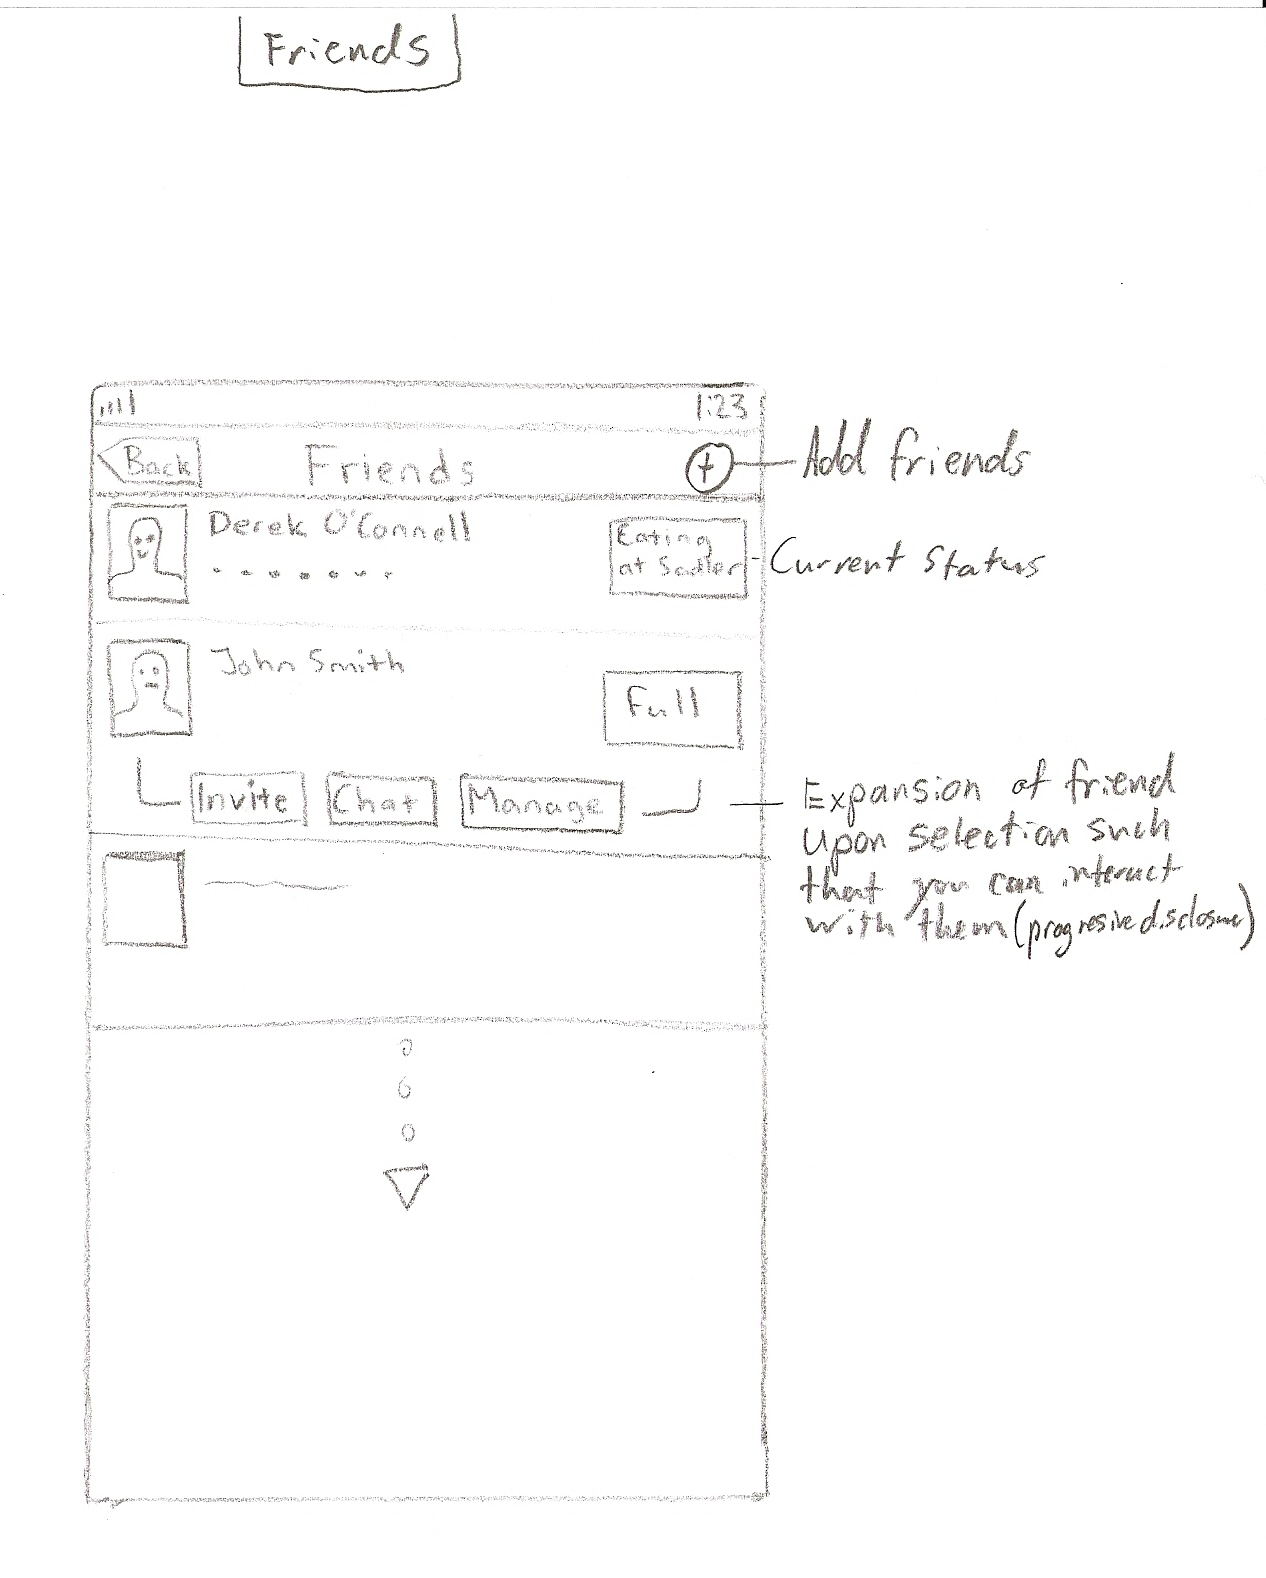
\includegraphics[width=0.8\linewidth]{team5.jpg}}
\caption{Friends Page}
\end{figure}

\begin{figure}[h!]
\centering
\fbox{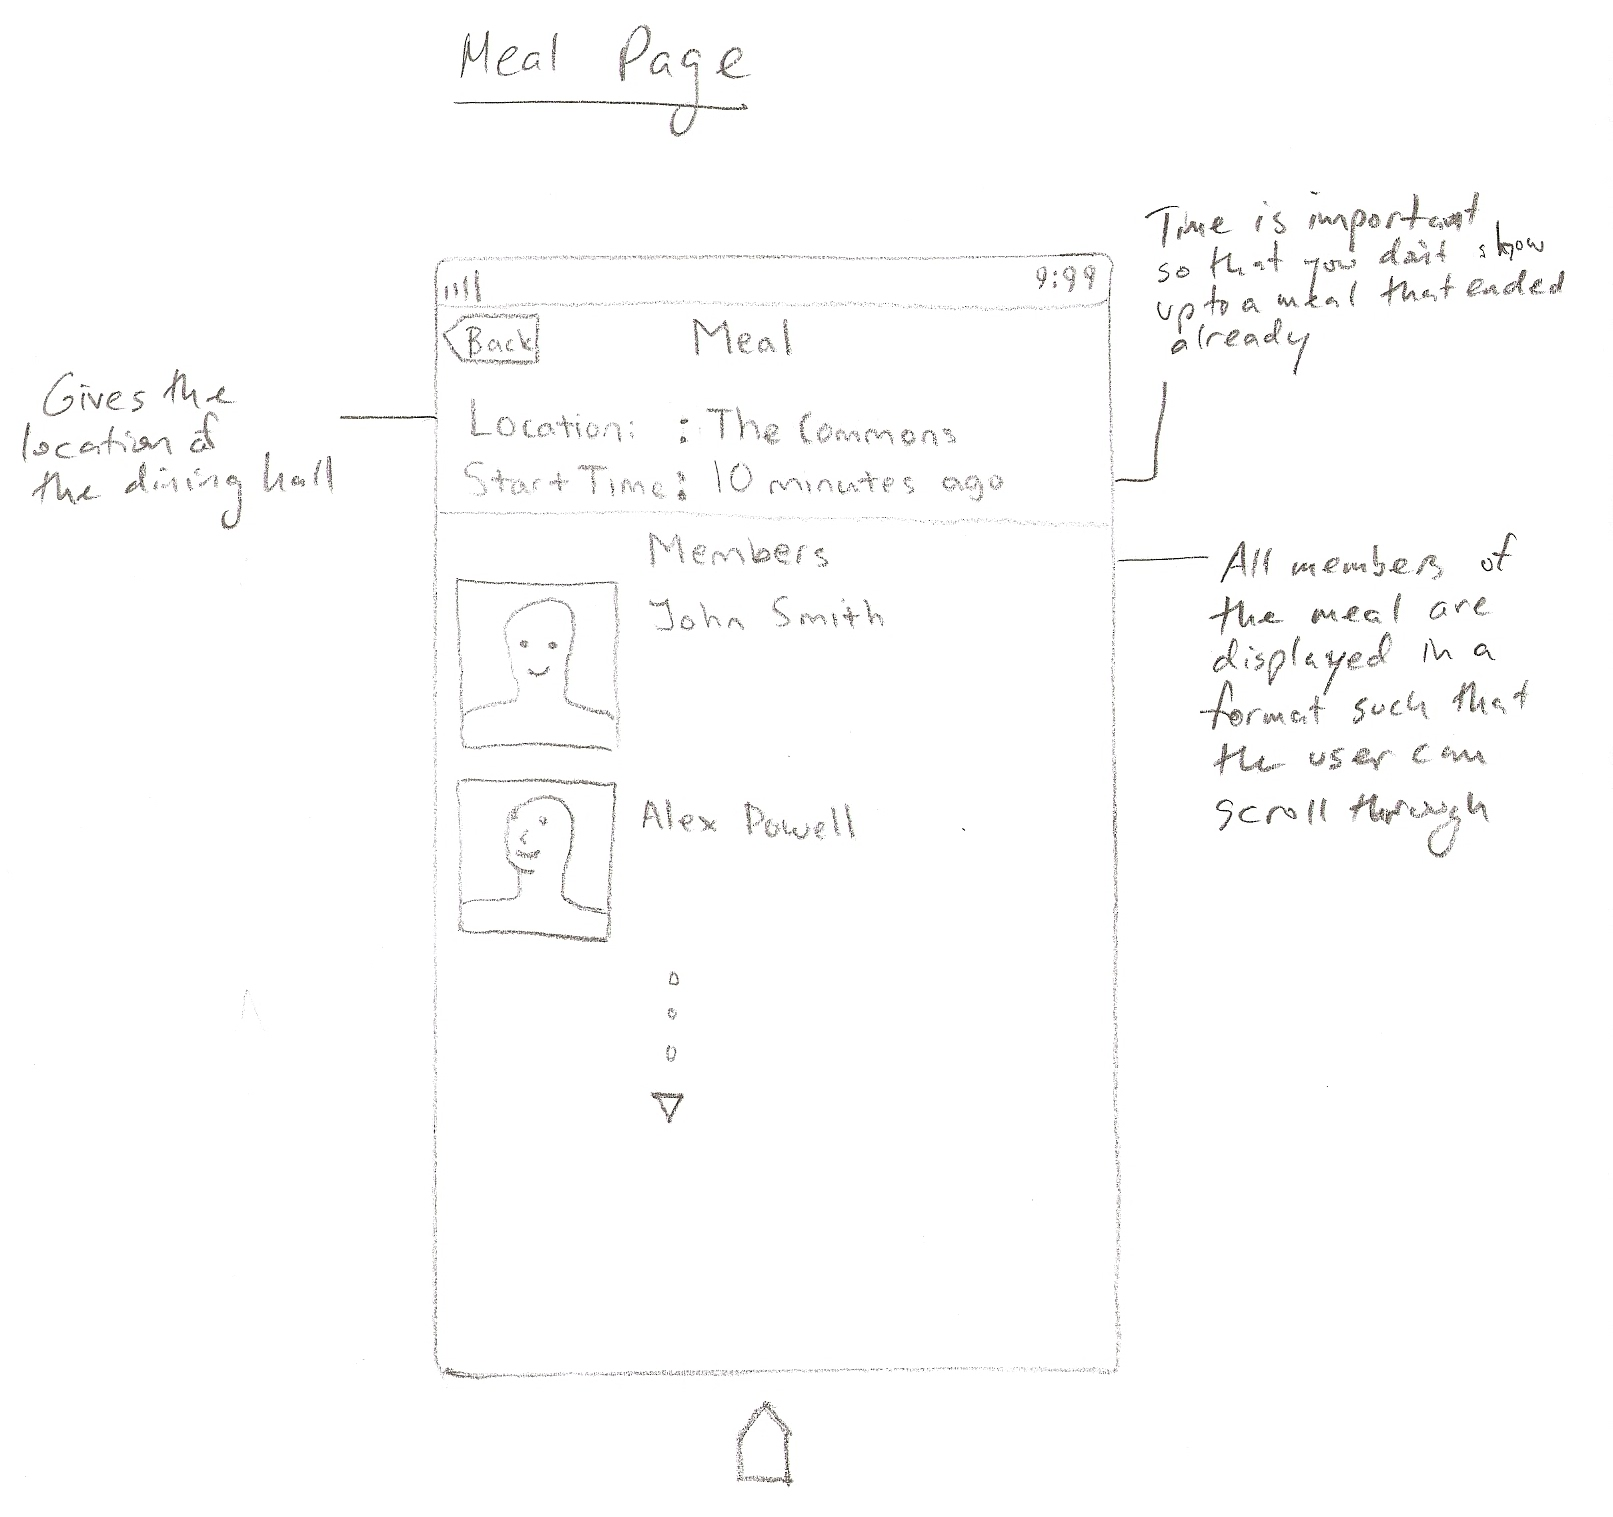
\includegraphics[width=0.8\linewidth]{team6.jpg}}
\caption{Meal Page}
\end{figure}

\clearpage
\section{User Journeys}

\begin{figure}[h!]
\centering
\fbox{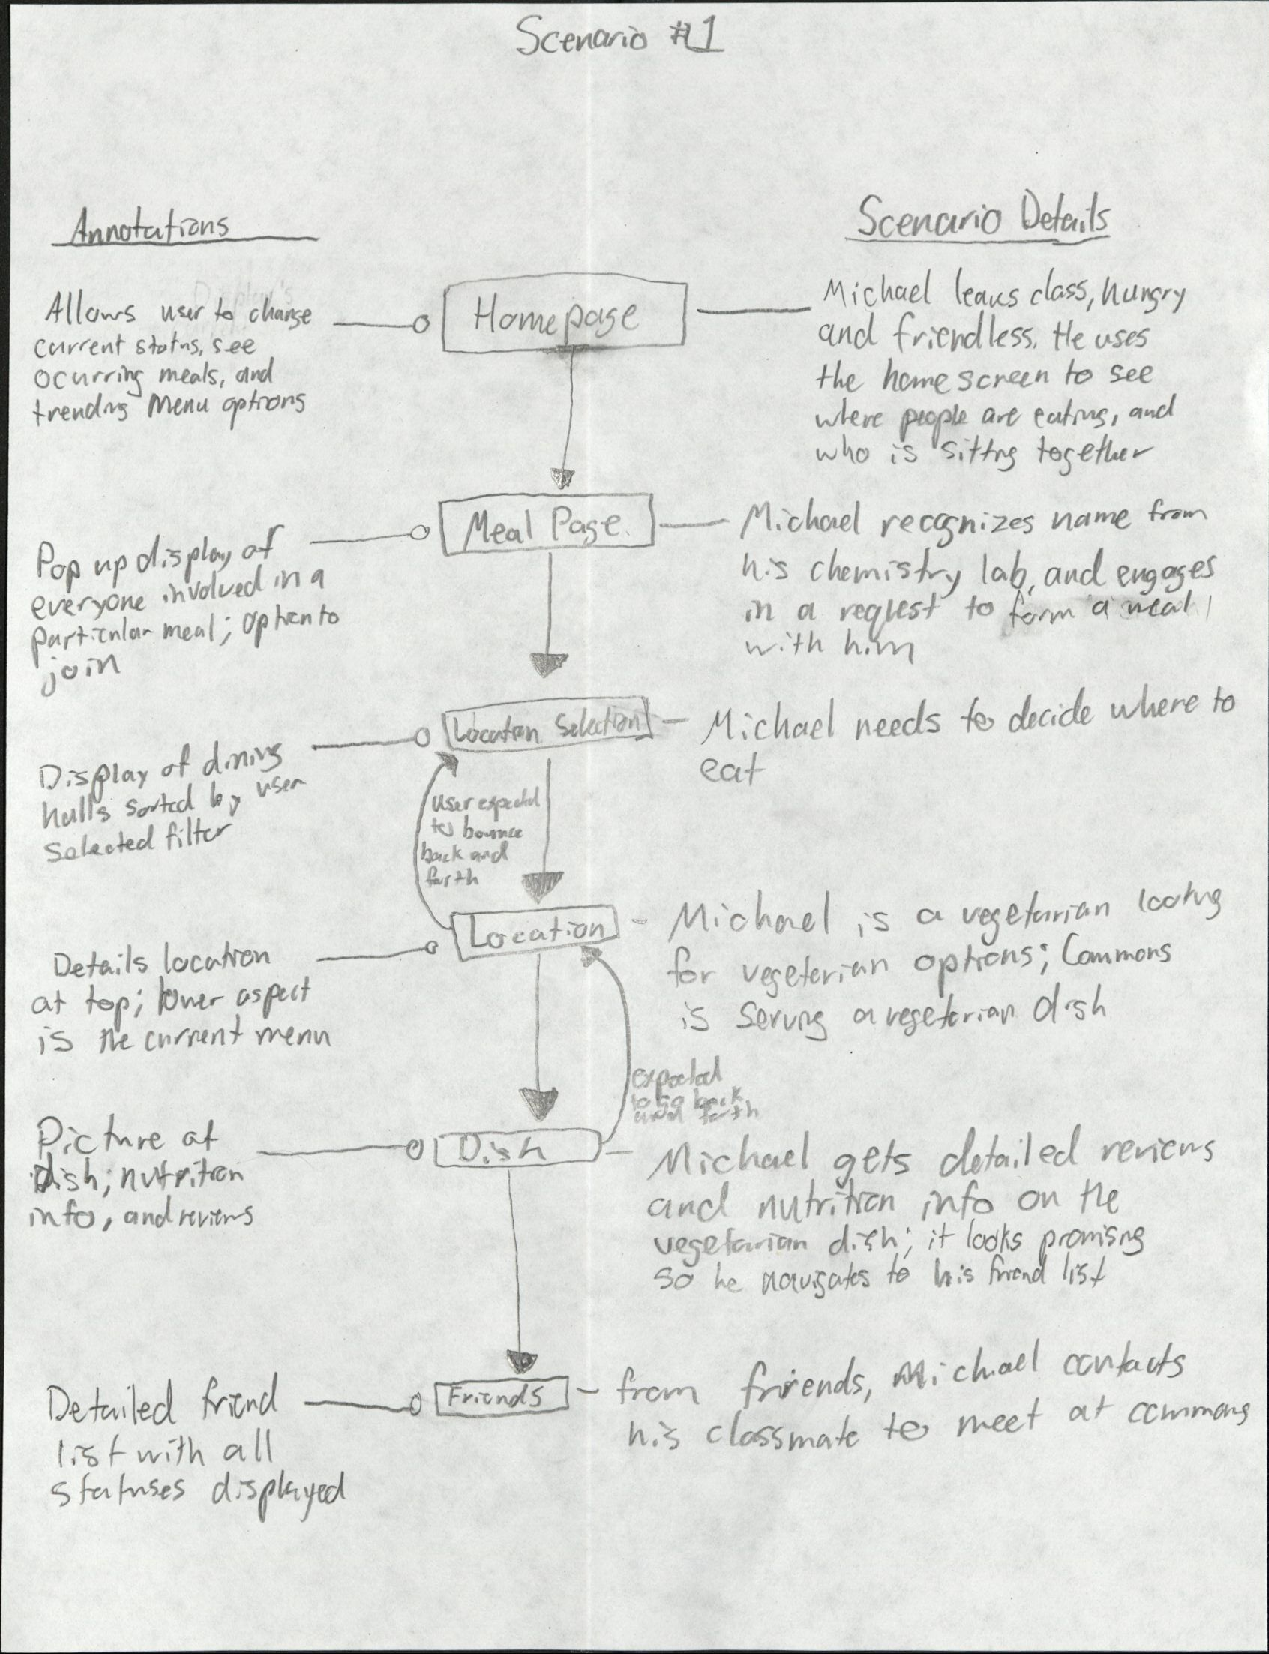
\includegraphics[width=0.8\linewidth]{user_journey1.pdf}}
\caption{User Journey for scenario 1}
\end{figure}

\begin{figure}[h!]
\centering
\fbox{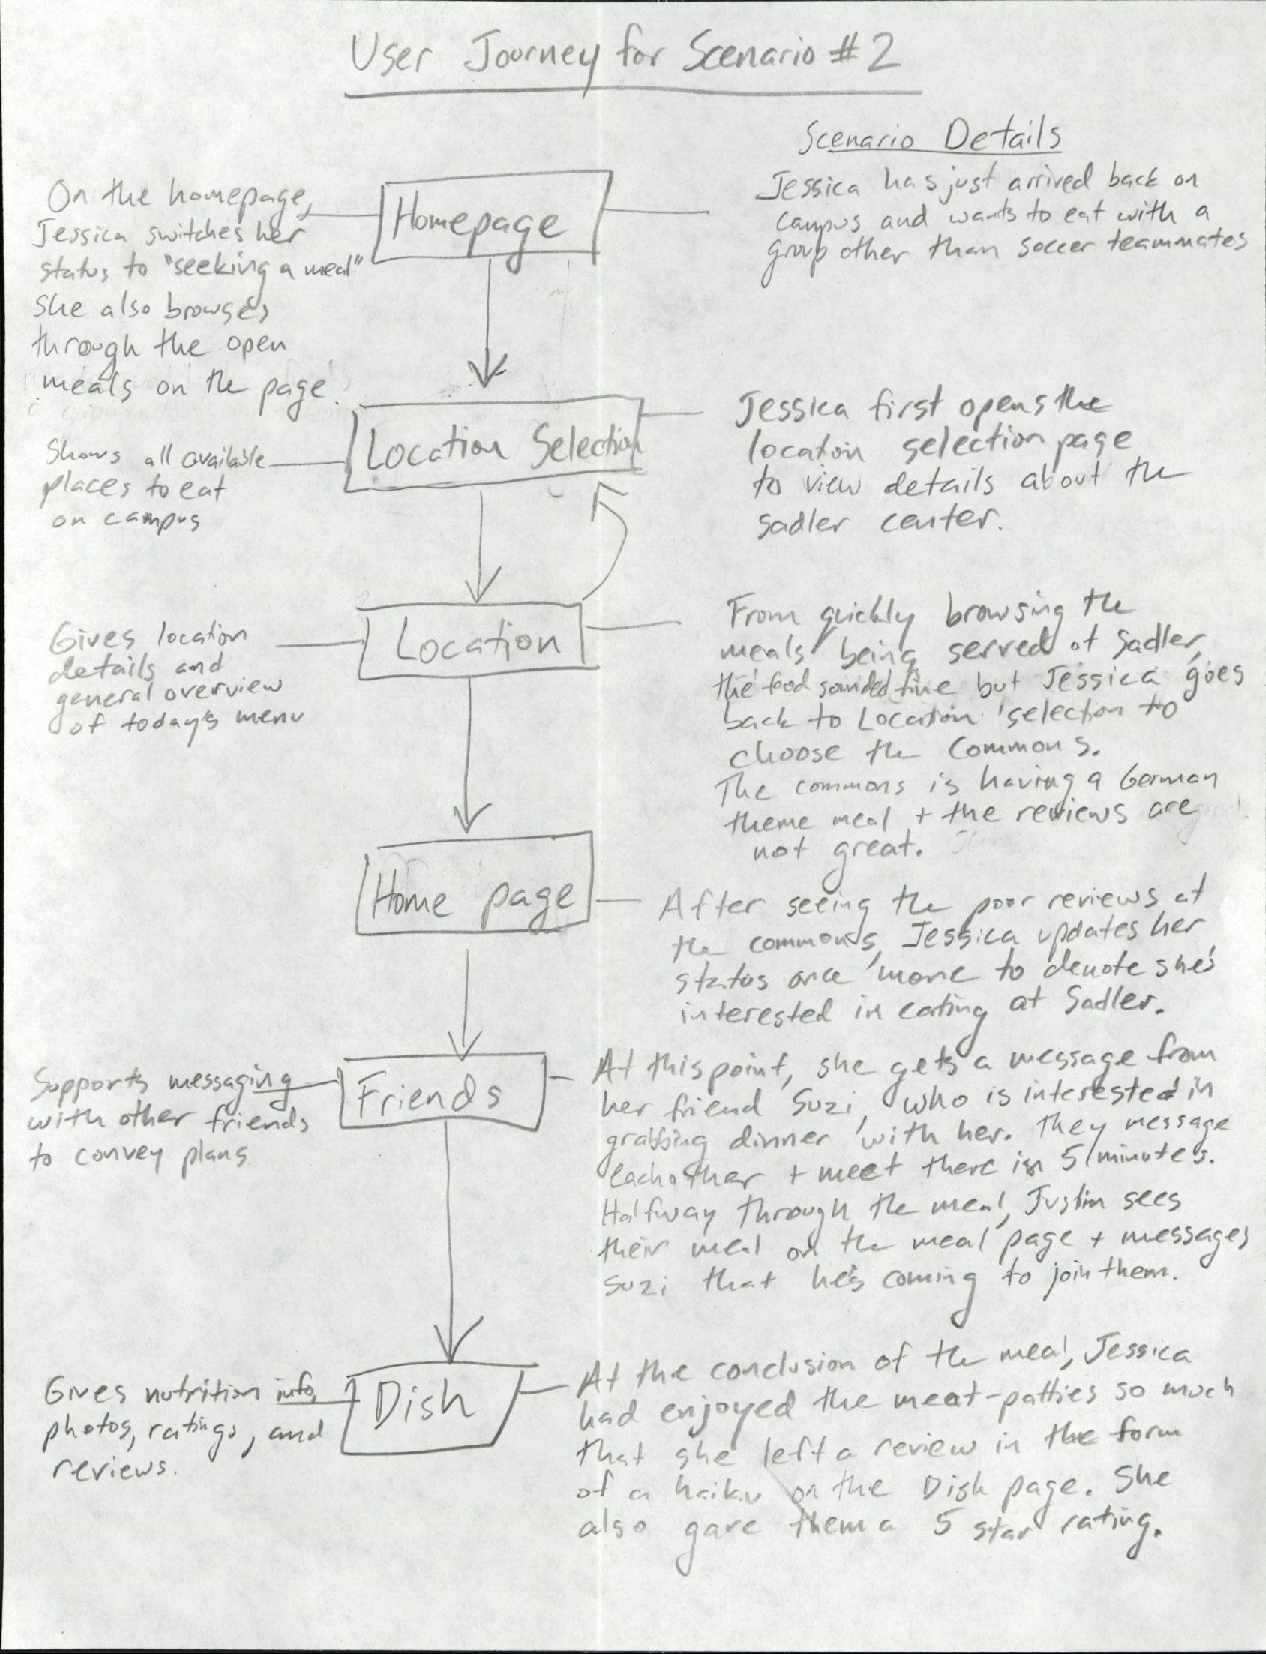
\includegraphics[width=0.8\linewidth]{user_journey2.pdf}}
\caption{User Journey for scenario 2}
\end{figure}

\clearpage
\section{Feedback from other students}
\begin{enumerate}
\item
\begin{itemize}
\item After speaking with several students, some noted that the home page seemed a little cluttered.  They noted that having two horizontal scrolling components on one page seemed a bit much.  Additionally, they raised concerns that the thumbnail images of the trending food on the home screen might be too small to be practical on most mobile phones.  When asked if they felt the same about the profile thumbnails directly above, they didn’t seem to view that as a concern, since the main goal of those components is to provide info about the number of participants in the meal.  
\item Another student noted that it might be more helpful and easier to use if we listed all reviews on the same page, but had the ability to sort by dining hall.  This is in contrast to the current system, which first requires the user to select a dining location and then navigates them to a new page to view reviews specific to that dining hall.  If they wanted to switch locations, they would have to press the back button, change the location preference, and re-enter the review hierarchy
\item A student also mentioned the fear of the app becoming overly social and inherently less informative due to its open nature. The particular student feared that the application may just turn into dining hall “bashing”, which could spin off into ridiculing individuals who are in charge of dining administration at the college. 
\item Initially, one student voiced concern that the social aspect was very similar with the app DownToLunch (one of our direct competitors), but after I showed him the menu and food review system he seemed to agree that there was a niche in the market for EatWithFriends.  
\item One concern mentioned by a pair of students concerned the privacy settings on the application. They feared that it might be too easy to inadvertently publicize their location and who they are with. This issue may have been avoided by providing a more comprehensive look at the settings screen, particularly those settings relevant to privacy. 
\end{itemize}
\item UX User Intervew \\
Name: Michael Wilkens \\
Social Class: Junior \\
Meal Plan: Block 100 \\
\begin{itemize}
\item Functionality:
\begin{itemize}
\item Concerned with who can see status/where eating
\item When writing reviews, who can see them? Who can write reviews?
\item On the location page, should be able to leave comments like: ‘crowded’, ‘broken ice cream machine’, anything not dish-specific
\item Could use location settings or check all existing meals to show how many people are at each dining hall
\item Also considered making pages for ‘eating’ locations like the terrace, where food isn’t sold people eat.
\item Wants to be able to post own pictures of food/dining hall
\item In the meal page, possibility to show how long the meal plans to go for
\item Have a meal-log where you can track what you eat
\item Give context for meals: intended length, plans afterward (go to library, go to sunken gardens)

\end{itemize}
\item UX:
\begin{itemize}
\item Pleased with layout of pages
\item Liked the idea of not having pages scroll two-dimensionally at the same time
\end{itemize}
\end{itemize}
\end{enumerate}

\end{document}





